    % Magda Gregorova, 2025-01-10
    % Non-binding template for MSc thesis in THWS/MAI submitted to Magda Gregorova
    % The template is provided "as is" without any guarantees.
    % You are free to use and modify as you see fit.

    \documentclass[12pt,twoside=false,a4paper,parskip,listof=totoc,appendixprefix=true,numbers=noenddot]{scrbook} % koma-script book environment for cleaner typesetting and more flexibility
    % \documentclass[12pt,twoside,a4paper,parskip,openright]{scrbook} % use this for double-sided printing

    %% ========== preamble ========== %%

    % Magda Gregorova, 2025-01-10
% example list of useful packages
% complement and adapt as you see fit

% text encoding
\usepackage[utf8]{inputenc} % standard text encoding
\usepackage[T1]{fontenc} % proper hyphenation of accented words
\usepackage{lmodern} % scalable Latin Modern fonts
\usepackage{microtype} % better line breaking
\usepackage[english]{babel} % typographical rules for English language
\usepackage{csquotes} % better handling of quotes (e.g. in refs.)
\usepackage[hidelinks]{hyperref} % cross-referencing for hypertext links

% pdf and page handling
\usepackage{pdfpages} % simplify insertion of external pdf pages
\usepackage{lscape} % for rotating pages to landscape
\usepackage{pdflscape} % pdf support for lscape
\usepackage{epstopdf} % convert eps to pdf

% floats, images, tables
\usepackage{graphicx} % \includegraphics with more options
\graphicspath{{./pics/}} % path to images
\usepackage{xcolor} % using colors
\usepackage{float} % better control of floats
\usepackage[verbose]{placeins} % correct placement of floats within sections (verbose logging)
\usepackage{wrapfig} % wrap text around figures
\usepackage{caption} % customize captions
\usepackage{subcaption} % sub-figures with sub-captions
\usepackage{multirow} % tables cells spanning multiple rows
\usepackage{longtable} % tables over several pages
\usepackage{booktabs} % improved tables
\usepackage{array}
\usepackage{tabularx}


% other goodies
\usepackage[shortlabels]{enumitem} % more control over layout of list environments
\usepackage[linesnumbered, boxed, resetcount]{algorithm2e} % for algorithms
\usepackage{listings} % for code listings

% compatibility with koma-script
\usepackage{scrhack} % compatibility package to emulate the former KOMA-Script
\usepackage[markcase=ignoreuppercase,headsepline,plainfootsepline]{scrlayer-scrpage} % manage page styles, markcase: automatic typesetting in heads, headsepline: line underneath the headerm, plainfootsepline: rule above the footer

% gantt chart
\usepackage{pgfgantt}


% tkiz
\usepackage{tikz}
\usetikzlibrary{positioning, arrows.meta}
\usepackage[edges]{forest}


% table


    % biblatex settings for better referencing
    \usepackage[backend=biber, % more flexible than bibtex
                % citestyle=authoryear,
                citestyle=numeric,
                % style=authoryear,
                style=numeric,
                sorting=none,
                maxbibnames = 10,
                % date = year,
                doi=false,
                isbn=false,
                url=false,
                eprint=false
                ]{biblatex}
    \DeclareDelimFormat{nameyeardelim}{\addcomma\space} % comma to separate name and year in cite command
    \addbibresource{references.bib} % your bibliography file
    \setcounter{biburllcpenalty}{7000} % allow line breaks in long URLs
    \setcounter{biburlucpenalty}{8000}
    \setcounter{biburlnumpenalty}{9000}

    % Magda Gregorova, 2025-01-10
% example list of custom commands to speed up typesetting frequent patterns
% complement and adapt as you see fit

\usepackage{amsmath,amsfonts,bm}
\numberwithin{equation}{chapter} % Number equations within a chapter

\DeclareMathOperator*{\argmax}{arg\,max}
\DeclareMathOperator*{\argmin}{arg\,min}

\newcommand{\norm}[1]{\left\lVert#1\right\rVert}%
\newcommand{\dN}{\mathcal{N}} % Normal distribution
\newcommand{\Ls}{\mathcal{L}} % Loss function

% Vectors
\def\vzero{{\bm{0}}}
\def\vone{{\bm{1}}}
\def\vmu{{\bm{\mu}}}
\def\vtheta{{\bm{\theta}}}
\def\vphi{{\bm{\phi}}}
\def\va{{\bm{a}}}
\def\vb{{\bm{b}}}
\def\vc{{\bm{c}}}
\def\vd{{\bm{d}}}
\def\ve{{\bm{e}}}
\def\vf{{\bm{f}}}
\def\vg{{\bm{g}}}
\def\vh{{\bm{h}}}
\def\vi{{\bm{i}}}
\def\vj{{\bm{j}}}
\def\vk{{\bm{k}}}
\def\vl{{\bm{l}}}
\def\vm{{\bm{m}}}
\def\vn{{\bm{n}}}
\def\vo{{\bm{o}}}
\def\vp{{\bm{p}}}
\def\vq{{\bm{q}}}
\def\vr{{\bm{r}}}
\def\vs{{\bm{s}}}
\def\vt{{\bm{t}}}
\def\vu{{\bm{u}}}
\def\vv{{\bm{v}}}
\def\vw{{\bm{w}}}
\def\vx{{\bm{x}}}
\def\vy{{\bm{y}}}
\def\vz{{\bm{z}}}

% Matrix
\def\mA{{\bm{A}}}
\def\mB{{\bm{B}}}
\def\mC{{\bm{C}}}
\def\mD{{\bm{D}}}
\def\mE{{\bm{E}}}
\def\mF{{\bm{F}}}
\def\mG{{\bm{G}}}
\def\mH{{\bm{H}}}
\def\mI{{\bm{I}}}
\def\mJ{{\bm{J}}}
\def\mK{{\bm{K}}}
\def\mL{{\bm{L}}}
\def\mM{{\bm{M}}}
\def\mN{{\bm{N}}}
\def\mO{{\bm{O}}}
\def\mP{{\bm{P}}}
\def\mQ{{\bm{Q}}}
\def\mR{{\bm{R}}}
\def\mS{{\bm{S}}}
\def\mT{{\bm{T}}}
\def\mU{{\bm{U}}}
\def\mV{{\bm{V}}}
\def\mW{{\bm{W}}}
\def\mX{{\bm{X}}}
\def\mY{{\bm{Y}}}
\def\mZ{{\bm{Z}}}
\def\mBeta{{\bm{\beta}}}
\def\mPhi{{\bm{\Phi}}}
\def\mLambda{{\bm{\Lambda}}}
\def\mSigma{{\bm{\Sigma}}}

% Random vectors
\def\rvepsilon{{\mathbf{\epsilon}}}
\def\rvtheta{{\mathbf{\theta}}}
\def\rva{{\mathbf{a}}}
\def\rvb{{\mathbf{b}}}
\def\rvc{{\mathbf{c}}}
\def\rvd{{\mathbf{d}}}
\def\rve{{\mathbf{e}}}
\def\rvf{{\mathbf{f}}}
\def\rvg{{\mathbf{g}}}
\def\rvh{{\mathbf{h}}}
\def\rvu{{\mathbf{i}}}
\def\rvj{{\mathbf{j}}}
\def\rvk{{\mathbf{k}}}
\def\rvl{{\mathbf{l}}}
\def\rvm{{\mathbf{m}}}
\def\rvn{{\mathbf{n}}}
\def\rvo{{\mathbf{o}}}
\def\rvp{{\mathbf{p}}}
\def\rvq{{\mathbf{q}}}
\def\rvr{{\mathbf{r}}}
\def\rvs{{\mathbf{s}}}
\def\rvt{{\mathbf{t}}}
\def\rvu{{\mathbf{u}}}
\def\rvv{{\mathbf{v}}}
\def\rvw{{\mathbf{w}}}
\def\rvx{{\mathbf{x}}}
\def\rvy{{\mathbf{y}}}
\def\rvz{{\mathbf{z}}}

% Random matrices
\def\rmA{{\mathbf{A}}}
\def\rmB{{\mathbf{B}}}
\def\rmC{{\mathbf{C}}}
\def\rmD{{\mathbf{D}}}
\def\rmE{{\mathbf{E}}}
\def\rmF{{\mathbf{F}}}
\def\rmG{{\mathbf{G}}}
\def\rmH{{\mathbf{H}}}
\def\rmI{{\mathbf{I}}}
\def\rmJ{{\mathbf{J}}}
\def\rmK{{\mathbf{K}}}
\def\rmL{{\mathbf{L}}}
\def\rmM{{\mathbf{M}}}
\def\rmN{{\mathbf{N}}}
\def\rmO{{\mathbf{O}}}
\def\rmP{{\mathbf{P}}}
\def\rmQ{{\mathbf{Q}}}
\def\rmR{{\mathbf{R}}}
\def\rmS{{\mathbf{S}}}
\def\rmT{{\mathbf{T}}}
\def\rmU{{\mathbf{U}}}
\def\rmV{{\mathbf{V}}}
\def\rmW{{\mathbf{W}}}
\def\rmX{{\mathbf{X}}}
\def\rmY{{\mathbf{Y}}}
\def\rmZ{{\mathbf{Z}}}


% Sets
\def\sA{{\mathbb{A}}}
\def\sB{{\mathbb{B}}}
\def\sC{{\mathbb{C}}}
\def\sD{{\mathbb{D}}}
% Don't use a set called E, because this would be the same as our symbol
% for expectation.
\def\sF{{\mathbb{F}}}
\def\sG{{\mathbb{G}}}
\def\sH{{\mathbb{H}}}
\def\sI{{\mathbb{I}}}
\def\sJ{{\mathbb{J}}}
\def\sK{{\mathbb{K}}}
\def\sL{{\mathbb{L}}}
\def\sM{{\mathbb{M}}}
\def\sN{{\mathbb{N}}}
\def\sO{{\mathbb{O}}}
\def\sP{{\mathbb{P}}}
\def\sQ{{\mathbb{Q}}}
\def\sR{{\mathbb{R}}}
\def\sS{{\mathbb{S}}}
\def\sT{{\mathbb{T}}}
\def\sU{{\mathbb{U}}}
\def\sV{{\mathbb{V}}}
\def\sW{{\mathbb{W}}}
\def\sX{{\mathbb{X}}}
\def\sY{{\mathbb{Y}}}
\def\sZ{{\mathbb{Z}}}



    %% ========== main part ========== %%
    \AtBeginBibliography{\renewcommand*{\finalnamedelim}{\addcomma\space}}
    \renewcommand*{\nameyeardelim}{\addcomma\space}
    \DefineBibliographyStrings{english}{andothers = {et\addabbrvspace al\adddot}}

    \begin{document}

    \frontmatter

    % Magda Gregorova, 2025-01-10
% standard title page

%% fill in your information
\def\ThesisAuthor{Fikrat Mutallimov}
\def\ThesisTitle{Comparative Analysis of SVG Deep Generative Models}
\def\SupervisorOne{Prof.\ Dr.\ Magda Gregorova}
\def\SupervisorTwo{Prof.\ Dr.\ -Ing. Erik Schaffernicht}
\def\SumbissionDate{April 14, 2026}

% for anonymous version
\def\iswithfullname{1} % comment this out to create anonymous version
\ifdefined\iswithfullname
  \def\ShowThesisAuthor{\ThesisAuthor}
\else
  \def\ShowThesisAuthor{N.~N.}
\fi

% metadata of pdf
\hypersetup{
pdfauthor={\ShowThesisAuthor},
pdftitle={\ThesisTitle},
}

% typsetting of titlepage
\titlehead{Technical University of Applied Sciences Würzburg-Schweinfurt (THWS)\\
Faculty of Computer Science and Business Information Systems}
\title{\ThesisTitle\\[15mm]}
\subject{Master Thesis}
\subtitle{{\normalsize submitted for the completion of degree} \\
\vskip 0.5cm
Master of Science \\
\vskip 0.2cm
in \\
\vskip 0.2cm
Artificial Intelligence
}
\author{\ShowThesisAuthor}
\date{\normalsize Submitted on: \SumbissionDate}
\publishers{\raggedright
  \normalsize{Supervisor: \SupervisorOne}\\
  \normalsize{Second Examiner: \SupervisorTwo}\\
}
\maketitle

    % Magda Gregorova, 2025-01-10
% abstract

\section*{Abstract (en)}
Current generative models can produce visually high-quality raster images from input
text or image, but the field falls short in vector graphics format due to its complex
nature. An SVG file is a document that contains paths, layers, and hierarchy and it
means its purpose is not just to represent something semantically, it should be structurally clean and neat. 
Those requirements create far more problems for 
building a model that generates SVG. This thesis analyzes SVG generation methods around thirteen recent models 
to understand how internal design choices affect the structure of output. The analysis is shaped around three dimensions, 
how models represent vector geometry internally, what supervision signals guide the generation process and which metrics 
are useful to evaluate the SVG. Representation and supervision interact rather than operate independently and they are two 
main parts of internal design of models. The analysis showed that the same loss function can produce different structural outcomes 
depending on the representation choice and the same representation behaves differently under different supervision. 
The most consistent pattern across the models is a trade-off between visual realism and editability. Models that generate the 
most visually detailed outputs also produce the most fragmented SVG files, while methods that constrain their representation 
or learn from data produce cleaner results, but within narrower domains. Current evaluation metrics (FID, CLIP, LPIPS) all operate 
on rendered pixels and cannot detect structural differences. To address this, the thesis proposes a six-dimension evaluation 
framework that includes path economy, geometric quality, layer organization, and editability alongside visual metrics. 
The thesis does not propose a new model. It provides a framework for understanding why current models produce the structures 
they do and what needs to change for generated SVGs to work in real design tools.


\section*{Abstract (de)}
Aktuelle generative Modelle können visuell hochwertige Rasterbilder aus Text oder Bildeingaben erzeugen, doch im Bereich der Vektorgrafiken bleibt das Feld aufgrund deren komplexer Natur zurück. Eine SVG-Datei ist ein Dokument, das Pfade, Ebenen und Hierarchie enthält, und das bedeutet, ihr Zweck ist nicht nur, etwas semantisch darzustellen, sondern sie muss auch strukturell sauber und ordentlich sein. Diese Anforderungen schaffen weit mehr Probleme, die es beim Bau eines Modells zur SVG-Generierung zu überwinden gilt. Die vorliegende Arbeit analysiert SVG-Generierungsmethoden anhand von dreizehn aktuellen Modellen, um zu verstehen, wie interne Entwurfsentscheidungen die Struktur der Ausgabe beeinflussen. Die Analyse ist um drei Dimensionen aufgebaut: wie Modelle die Geometrie von Vektorgrafiken intern repräsentieren, welche Supervisionssignale den Generierungsprozess leiten und welche Metriken zur Bewertung der SVG nützlich sind. Repräsentation und Supervision wirken zusammen statt unabhängig voneinander und sind die zwei Hauptbestandteile des internen Designs der Modelle. Die Analyse hat gezeigt, dass dieselbe Verlustfunktion unterschiedliche strukturelle Ergebnisse erzeugen kann, je nach Repräsentationswahl, und dieselbe Repräsentation sich unter verschiedener Supervision unterschiedlich verhält. Das konsistenteste Muster über die Modelle hinweg ist ein Kompromiss zwischen visuellem Realismus und Editierbarkeit. Modelle, die visuell besonders detaillierte Ausgaben erzeugen, produzieren gleichzeitig die fragmentiertesten SVG-Dateien, während Methoden, die ihre Repräsentation einschränken oder aus Daten lernen, sauberere Ergebnisse liefern, jedoch innerhalb engerer Domänen. Aktuelle Evaluierungsmetriken (FID, CLIP, LPIPS) arbeiten ausschließlich auf gerenderten Pixeln und können strukturelle Unterschiede nicht erkennen. Um dies zu adressieren, schlägt die Arbeit ein sechsdimensionales Evaluierungsframework vor, das Pfadökonomie, geometrische Qualität, Ebenenorganisation und Editierbarkeit neben visuellen Metriken einbezieht. Die Arbeit schlägt kein neues Modell vor. Sie liefert einen Rahmen, um zu verstehen, warum aktuelle Modelle die Strukturen erzeugen, die sie erzeugen, und was sich ändern muss, damit generierte SVGs in realen Designwerkzeugen funktionieren.

\newpage
\chapter*{Acknowledgment}
I want to thank Prof. Dr. Magda Gregorova and Philipp Vaeth for supervising this thesis.
At the beginning of the process, I had no clear direction and their guidance 
is what kept me focused and moving forward. 
Every session gave me something concrete to work with. 
I am also grateful for the freedom they gave me to shape the analytical approach on my own terms.

I thank Prof. Dr. Erik Schaffernicht, as second examiner.

I thank Shabnam Huseynova for her support during the thesis period.

Special thanks to Ismail Eyyublu, a designer at McKinsey in Baku, 
who helped me understand SVG from the perspective of someone who actually works with it. 
His explanations of what designers expect from generated vector graphics shaped 
how I thought about editability throughout this thesis.


AI language model Claude (Anthropic)~\cite{claude2026} was used during the preparation of this thesis for brainstorming, literature comprehension, 
text editing, and translation. 


    \tableofcontents

    \mainmatter

    \chapter{Introduction}
\label{ch:Introduction}

Vector graphics differ fundamentally from raster images.
Raster images represent visual content as grids of pixels, 
where each pixel stores color information independently of its neighbors. 
Vector graphics instead describe images using mathematical primitives: 
lines, curves, shapes, and groups defined parametrically. 
Because the geometry is encoded, rather than sampled, vector graphics scale without loss 
and can be edited at the level of individual components. 
Among vector formats, Scalable Vector Graphics (SVG) has become 
the dominant web standard. Its structured nature makes it programmable: 
SVG files can be generated, modified, and animated through code, 
which is why the format underlies most of what is drawn on the web. 
A 2024 survey by W3Techs found that over 65\% of all websites use SVG for their graphics~\cite{w3techsSVG2024}.

In terms of generative modelling,
the structure of SVG introduces challenges that do not arise in raster synthesis.
SVG graphics encode both geometry and topology. 
So a generated SVG must satisfy two requirements simultaneously: 
it must look correct and it must be structurally clean. 
Although it may seem visually plausible, an output with redundant paths 
and unstable geometry cannot be edited or reused. 
Visual quality and structural quality are distinct properties, 
and current evaluation practice does not consistently distinguish between them.

Before learning-based approaches, vector graphics were 
produced through algorithmic vectorization: tools that 
approximate raster images using geometric primitives 
via edge detection, contour tracing, and polygon 
approximation. These methods remain in use 
but rely on heuristic rules and struggle with complex 
scenes. Learning-based approaches introduce new 
possibilities, but also raise questions about how 
models construct vector structure internally and 
whether the outputs they produce are usable in practice.


\section{Motivation}
\label{sec:motivation}

In recent years, generative models have substantially changed what 
is possible in visual content creation. Diffusion models, large-scale 
multimodal systems, and transformer based architectures have demonstrated 
that high-quality image synthesis from text prompts is no longer 
a research prototype. Systems such as Stable Diffusion, DALL-E, and 
Midjourney produce raster images that are often indistinguishable from 
photographs or hand-drawn illustrations. Progress in this area has been 
fast. But this progress has not extended equally to vector graphics. 
Research on SVG generation has grown, but the reliability and structural 
quality of generated outputs remain open problems. It is worth considering that 
vector graphics have not become less important. Instead, icons, logos, 
interface elements, illustrations, and data visualizations are created 
and maintained in vector formats precisely because they remain editable 
and resolution-independent. The formats used by Adobe Illustrator, 
Figma, and every major web browser are vector-based.



The gap between raster and vector generation is not only technical 
difficulty. It reflects a mismatch between how 
generative models are trained and evaluated and what vector graphics 
actually require. A model trained to minimize pixel reconstruction error 
has no reason to produce clean paths or interpretable layers or a model 
evaluated by FID score is rewarded for visual plausibility, not 
structural usability. Those are just a few examples, and we will see 
more of them later. It is understandable, because early generative 
models focused on raster images which led the vector graphics 
field to be partially dependent on raster images and their features. 
But still there are different methods and techniques used to generate 
SVG. Rather than proposing a new 
generation model, this thesis analyzes existing methods from the inside: 
how they represent vector graphics, what supervision signals they use, 
and how those choices shape the structure of the outputs they generate.

\section{Research Problem}

SVG generation research has divided across different directions. 
Some models treat SVG as a stream of drawing commands, other approaches
refine vector parameters directly against a raster target.
It is even possible to define geometry through learned functions. 

These methods differ not only in architecture but in how they internally 
represent vector structure and what signals they use to guide generation.
Despite this diversity, a systematic understanding of how these design 
choices influence the structure of what gets produced is missing. 
Models use different representations, different supervision signals, 
and different optimization strategies, but no existing work traces 
how those choices connect to the structural properties of the output. 
Two models may achieve similar FID scores while producing outputs with 
completely different path counts, layer organization, and editability. 
The field has many methods but no shared framework for understanding why 
they produce the structures they do.

Evaluation makes this harder. The metrics most commonly used 
(FID, LPIPS, CLIP score) are all borrowed from raster synthesis and 
operate on rendered pixels. They cannot detect redundant paths, broken 
hierarchy, or unusable geometry. There is no widely adopted benchmark 
for SVG editability, path economy, or layer coherence.
This combination --- heterogeneous architectures, 
untraced design-to-structure relationships, and evaluation that ignores 
structure --- constitutes the research gap addressed by this thesis.

\section{Thesis Objective}
\label{sec:objective}

This thesis investigates SVG generation methods from 
the perspective of representation, supervision, and 
structural quality. The goal is not to propose a new 
model but to develop a structured analytical 
understanding of how existing methods construct vector 
graphics and why their structural outcomes differ.

The analysis focuses on models where the generation 
process is interpretable in terms of vector operations 
or clearly defined architectural components. Large 
language model approaches, which treat SVG generation 
as code synthesis, are reviewed as a distinct and 
growing direction but excluded from the main analysis. 
A full justification is 
provided in Appendix~\ref{app:llm_exclusion}.

The thirteen models in the main analysis were selected 
by a few practical criteria, and the selection is not 
exhaustive. Each one is a recent method (2020 to 2025) 
that uses differentiable rendering or learned models and 
produces SVG or structured vector output. Each paper also describes its architecture in 
enough detail to analyze how the model represents 
geometry and how it is supervised. The models were 
chosen so that together they cover the different 
representation and supervision types. Whether code is 
publicly available was recorded 
(Table~\ref{tab:reproducibility}), but it was not a 
requirement.


\section{Research Goals}

\begin{enumerate}
    \item To explain and analyze the core properties, 
    structures, and components of SVG graphics as a 
    foundation for understanding their representation 
    and generation.
    \item To collect, review, and categorize a 
    representative set of existing methods for SVG 
    generation across different input modalities.
    \item To investigate the deep learning architectures 
    employed in SVG generation models and analyze their 
    design principles.
    \item To examine how these architectures represent 
    SVG data internally and how outputs are transformed 
    into standard SVG files.
    \item To evaluate existing approaches, metrics, and 
    benchmarks for assessing the quality of generated 
    SVGs.
    \item To assess and compare the structural and visual 
    quality of current SVG generation models based on 
    identified evaluation criteria.
\end{enumerate}


\section{Research Questions}

\begin{enumerate}
    \item What are the main properties and structures 
    that define an editable and high-quality SVG?
    \item What methods currently exist for 
    generating SVGs from different input modalities?
    \item What types of deep learning architectures are 
    used in SVG generation models?
    \item What kinds of structure do these models produce?
    \item How can the quality and editability of generated 
    SVG be evaluated?
    \item What is the reported and assessed quality of 
    SVG outputs across different models?
\end{enumerate}

These questions are not independent. Together they 
form a single analytical inquiry: how do the internal 
design choices of SVG generation models (what they 
represent, how they are supervised, and how their 
outputs are evaluated) determine whether the resulting 
graphics are structurally usable as well as visually 
plausible. The thesis argues that this question cannot 
be answered by visual metrics alone, and that 
systematic analysis of representation and supervision 
is necessary to explain the structural differences 
observed across current methods.


\section{Thesis Structure}

Chapter~\ref{ch:Background} 
introduces the foundational concepts required to understand 
vector graphics generation: SVG structure, representation 
types, differentiable rendering, and the supervision 
strategies used in learning-based methods.
Building on this, Chapter~\ref{ch:Landscape} surveys 
existing SVG generation approaches and categorizes 
them by architectural family and input modality. 
Chapters~\ref{ch:representation} and~\ref{ch:supervision} 
analyze how representation and supervision choices 
shape vector structure, tracing the relationship 
between internal design decisions and observable 
output properties.
Chapter~\ref{ch:Evaluation} introduces a 
multi-dimensional evaluation framework for SVG 
generation that extends beyond visual similarity to 
include structural and practical criteria. These 
perspectives are then applied in 
Chapter~\ref{ch:synthesis}, where strengths, 
limitations, and trade-offs across the analyzed 
models are examined comparatively.
The thesis concludes by mapping findings to the 
research questions, summarizing contributions, and 
identifying directions for future work.






    \chapter{Background}\label{ch:Background}

Generating vector graphics computationally is harder than 
it seems. Unlike raster images, which can be produced by 
predicting pixel values, SVGs have to be 
structurally correct and the resulting file needs 
to be something a designer can actually open and work with. Otherwise,
the output is not really something that can be used in practice.   
Getting there requires understanding the building 
blocks that most SVG generation models have in common, 
despite the variety of approaches and architectures that exist. 
This chapter covers those building blocks. It starts with 
SVG itself: what the format represents, how it is structured, 
and why those structural properties create constraints that 
raster generation does not have. From there it introduces 
four internal representation types used across the analyzed 
models, then differentiable rendering, which is the technical 
bridge that connects vector parameters to pixel-space losses. 
The chapter closes with the supervision signals (reconstruction 
losses, CLIP, SDS, VSD) that drive the generation process in 
different ways.

\section{Vector Graphics Fundamentals}
\label{sec:vector_fundamentals}

Scalable Vector Graphics (SVG) is an XML-based standard for 
representing two-dimensional graphics as structured 
text~\cite{eisenbergSVGEssentialsProducing20}. The difference between raster formats and SVG 
is that an SVG file is a readable document that describes how an image should 
be drawn rather than storing pixel values. At its core, an SVG file consists of instructions or commands that 
define geometric primitives such as circles, rectangles, lines, and 
paths, along with styling and hierarchical relationships between 
elements~\cite{quintScalableVectorGraphics2003}.

SVG supports a range of graphic elements, including basic shapes 
such as lines, rectangles, and circles, as well as text and 
raster images. The most flexible element is the path, 
which allows complex shapes to be defined using sequences of 
commands: moving a virtual pen, drawing straight lines, and 
creating smooth curves~\cite{eisenbergSVGEssentialsProducing20}.

What makes SVG practically useful is editability, and that 
editability comes from groups and layers. Multiple shapes can be combined into groups that behave as a 
single unit for styling and editing~\cite{quintScalableVectorGraphics2003}. 
Elements are rendered in a defined order, and later elements 
appear on top of earlier ones, making layering an intrinsic 
part of the representation. This hierarchical structure is what makes SVG files 
editable in practice: a designer can select a group, 
move a layer, or change one element without affecting 
the rest.

Figure~\ref{fig:svg_example} shows a minimal SVG file and 
its rendered output. The file is plain text: each element 
is a single readable line that defines geometry and color 
directly. This is what makes SVG editable. A designer 
can open the file, find the element they want, and change 
a number.

\begin{figure}[htbp]
\centering
\begin{minipage}{0.52\textwidth}
\begin{lstlisting}[language=XML, basicstyle=\small\ttfamily, showstringspaces=false]
<svg xmlns="http://www.w3.org/2000/svg"
     width="200" height="200">
  <!-- Face -->
  <circle cx="100" cy="100" r="80"
          fill="#FFD700"/>
  <!-- Left eye -->
  <circle cx="70" cy="80" r="10"
          fill="#333"/>
  <!-- Right eye -->
  <circle cx="130" cy="80" r="10"
          fill="#333"/>
  <!-- Sad mouth -->
  <path d="M 65 135 Q 100 110 135 135"
        stroke="#333" stroke-width="5"
        fill="none"/>
</svg>
\end{lstlisting}
\end{minipage}
\hfill
\begin{minipage}{0.40\textwidth}
\centering

\includegraphics[width=\textwidth]{simpleSVG.png}
\end{minipage}
\caption{A minimal SVG file (left) and its rendered output 
(right). Each element is one readable line: the face, 
eyes, and mouth are independent objects defined by plain 
text parameters. Any of them can be selected and changed 
without touching the rest.}
\label{fig:svg_example}
\end{figure}

\subsection{Paths and Bézier Curves}

Most SVG graphics are built using paths. A path is a sequence 
of commands (\emph{move to}, \emph{line to}, \emph{curve to}) 
that define its 
shape~\cite{eisenbergSVGEssentialsProducing20}. Curved segments 
use B\'{e}zier curves, which are not defined by the points they 
pass through but by control points that pull the curve toward 
them from the outside. Moving a control point reshapes the curve 
smoothly without breaking it.

As shown in Figure~\ref{fig:bezier}, SVG supports two types. 
Quadratic B\'{e}zier curves use a single control point and 
are simpler but less flexible. Cubic B\'{e}zier curves use 
two control points and can represent almost any smooth 
shape~\cite{eisenbergSVGEssentialsProducing20}. Most 
generation models in this thesis work with cubic curves 
because they are expressive enough to approximate complex 
geometry. The control point coordinates are the core 
parameters that models either predict directly or adjust 
during optimization.

\begin{figure}[htbp]
\centering
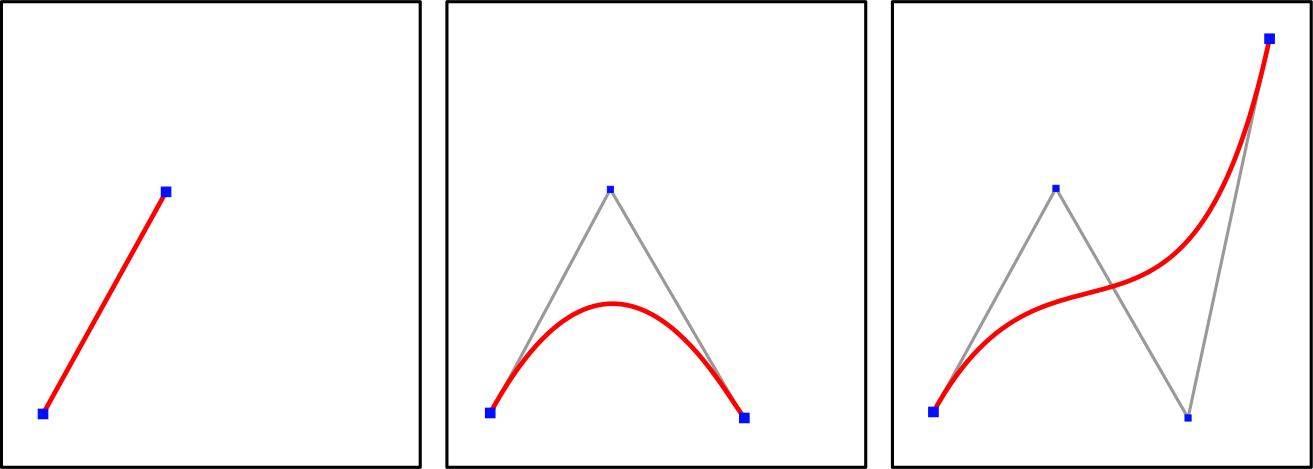
\includegraphics[width=0.85\textwidth]{Bezier_grad123.png}
\caption{B\'{e}zier curves of degree 1, 2, and 3 (red) with 
their control polygons (gray). From left to right, an 
additional control point (blue) is added at each degree. 
The curve changes direction and curvature as control points 
are inserted or moved. Image: Wikimedia 
Commons~\cite{wikiBezier}.}
\label{fig:bezier}
\end{figure}



\subsection{Coordinate Systems and Transformations}

SVG uses a simple coordinate system. The top-left corner of 
the canvas is the origin, x increases to the right, and y 
increases downward~\cite{quintScalableVectorGraphics2003}. 
Every element is positioned within this grid using numeric 
coordinates, the same numbers you see in the SVG file.

What makes this system powerful for design is transformations. 
Any shape or group can be moved, scaled, rotated, or skewed 
by applying a transform attribute. When a transformation is 
applied to a group, every element inside moves together. 
Groups can be nested inside other groups, each with their 
own local coordinate frame. A logo might have a top-level 
group for the whole graphic, sub-groups for each component, 
and individual paths inside those. Moving the top-level group 
moves everything. Moving a sub-group moves only that part. 
This nested structure is what allows complex SVG files to 
remain organized and editable even as they grow in size.



\section{Vector Representations}

SVG generation and vectorization models do not all manipulate 
vector graphics the same way internally in generation processes. Obviously, the final output is 
always a text-based file or SVG itself as image. What differs is the internal representation 
used during learning or optimization. This choice directly 
affects which algorithms can be applied, how stable training 
is, what structural properties tend to emerge and the quality of final output. 
The following sections introduce the four representation types 
that appear across the models analyzed in this thesis.

\subsection{Parametric Representation}
\label{sec:parametric_repr}

Parametric representation is natural for SVG because  
SVG is already parametric. Every element in the file is 
defined by control point coordinates, stroke 
widths and colors which are readable and editable as plain 
text~\cite{eisenbergSVGEssentialsProducing20}. The introduction 
of differentiable rasterization by Li et 
al.~\cite{liDifferentiableVectorGraphics2020a} made it practically possible 
to optimize these parameters directly using image-based loss 
functions: a graphic is initialized as a collection of 
primitives, and their parameters are iteratively refined until 
the rendered output matches a target.

\subsection{Sequential Representation}
\label{sec:sequential_repr}

The idea of treating vector graphics as ordered sequences of 
drawing commands goes back to SketchRNN by Ha and 
Eck~\cite{haNeuralRepresentationSketch2017}, who showed that 
recurrent networks could learn to generate stroke-based 
drawings by modelling them as sequences of pen movements. 
Vector graphics encoded this way look like a script: move the pen here,
draw a line there, curve to this point. These representations share the same basic 
structure as a sentence, which opened the door to applying 
language modelling techniques directly. The downside of that approach 
is that whenever errors accumulate, a mistake early in a long sequence can 
break everything that follows.

\subsection{Implicit Neural Representation}
\label{sec:implicit_repr}

The use of neural networks to define geometry implicitly 
through learned weights was established in 
3D scene representation by Mildenhall et 
al.~\cite{mildenhallNeRFRepresentingScenes2020}. In NeRF,
the network acts like a function: based on a given location,
it tells you what occupies that 
space. Nothing is stored explicitly, the geometry 
only appears when you query the network.
Thamizharasan et 
al.~\cite{thamizharasanNIVeLNeuralImplicit2024} adapted this 
idea to vector graphics by replacing explicit path coordinates 
with neural implicit layers that define shape boundaries 
indirectly. The network learns to represent the geometry as a continuous 
function and the resulting shapes emerge from the learned implicit representation 
instead of being directly parameterized. This allows for more flexible and 
compact representations, but also makes it harder to control specific 
geometric features directly, because they are not explicitly defined as 
parameters.   

Take the mouth 
in Figure~\ref{fig:svg_example}, \texttt{M 65 135 Q 100 110 135 135}. 
A parametric representation stores its three points directly: start 
(65,~135), control point (100,~110), and end (135,~135), plus stroke 
width and color. Optimization changes these numbers. A sequential 
representation turns the same curve into tokens: a move command with 
the arguments 65 and 135, then a quadratic curve command with 100, 110, 
135, and 135. The model has to predict them in that order. An implicit 
representation like NeuralSVG stores none of these numbers. The mouth 
is simply shape number 4. The MLP takes the index 4 as input and 
outputs the control points and the color of that 
shape~\cite{polaczekNeuralSVGImplicitRepresentation2025}. To change 
the mouth, you change the network weights, and the numbers only appear 
when the network is queried. NIVeL works the other way around: its network 
takes a pixel coordinate and returns which layer covers it, so the 
curve only appears after it is traced from the 
field~\cite{thamizharasanNIVeLNeuralImplicit2024}.


\subsection{Latent Space as a Generative Layer}
\label{sec:latent_repr}

Latent representation is not a geometric representation at all. 
It is a generative layer that sits on top of one of the other three.
There are no control points, no path commands, no shape boundaries 
stored anywhere. Latent space compresses many graphics
into a shared numerical embedding learned during training. 
Kingma and Welling~\cite{kingmaAutoEncodingVariationalBayes2022} 
formalized this idea through the Variational Autoencoder: 
an encoder compresses an input into a short vector and a 
decoder reconstructs the original from it.

For SVG generation, the actual geometry is always produced 
by the decoder, which translates a latent vector back into 
one of the other representation types: parametric paths or sequential commands.
The latent space sits on top as an organizational layer. It is included 
here because several models use it this way and confusing 
it with a geometric representation leads to misunderstanding 
how those models actually construct their outputs.



\section{Differentiable Rendering}
\label{sec:diffvg}

DiffVG~\cite{liDifferentiableVectorGraphics2020a} is one of the main bridges between vector and pixel spaces. 
Before neural networks can optimize vector graphics using 
image-based loss functions, there needs to be a way to connect 
the two spaces. Vector parameters (control points, stroke widths, colors) live
in a continuous geometric space. Loss 
functions operate on pixel values. These two spaces are not 
naturally connected: traditional rasterization converts vector 
geometry into pixels, but this process is not differentiable, 
meaning gradients cannot flow back through it to update the 
vector parameters.

DiffVG, introduced by Li et al.~\cite{liDifferentiableVectorGraphics2020a}, 
solves this by approximating rasterization in a way that 
supports gradient computation. Given a set of vector 
parameters as input, DiffVG renders a pixel image as output. 
Because the rendering step is differentiable, the loss computed 
on the output image (whether a pixel reconstruction loss,
a perceptual loss, or a signal from a pretrained semantic model) 
can be backpropagated all the way through to the 
vector parameters themselves. The system learns which control 
point to move, and in which direction, to reduce the error. 
The tricky part is handling edges and anti-aliasing, places 
where a tiny shift in a path boundary causes a sudden pixel 
change. DiffVG approximates these discontinuities in a way 
that still produces usable gradients~\cite{liDifferentiableVectorGraphics2020a}.

Before DiffVG, optimizing vector graphics with gradient-based 
methods was not straightforward. Its introduction made it 
possible to apply the full range of image-based supervision 
strategies, reconstruction losses, CLIP guidance, diffusion 
priors directly to vector parameters.

The core idea is shown in Figure~\ref{fig:diffvg_pipeline}. 
Normally, converting vector shapes to pixels is a one-way 
street: you can go from shapes to pixels, but not back. 
DiffVG makes the middle step reversible. Once gradients 
can flow back through the rasterizer, any image-based loss 
function becomes usable for optimizing vector parameters 
directly.

\begin{figure}[htbp]
\centering
\begin{tikzpicture}[
  box/.style={rectangle, draw, rounded corners,
              minimum width=2cm, minimum height=0.8cm,
              text centered, font=\small, fill=gray!10},
  arrow/.style={->, thick}
]
\node[box] (params) at (0,0)   {SVG Params};
\node[box] (diffvg) at (3,0)   {DiffVG};
\node[box] (image)  at (6,0)   {Pixel Image};
\node[box] (loss)   at (9,0)   {Loss};

\draw[arrow] (params) -- (diffvg);
\draw[arrow] (diffvg) -- (image);
\draw[arrow] (image)  -- (loss);
\draw[arrow] (loss) to[bend right=40] 
    node[below, font=\scriptsize] {gradients flow back} (params);
\end{tikzpicture}
\caption{The differentiable rendering pipeline. DiffVG 
converts vector parameters into a pixel image. A loss 
compares this image to a target. Gradients then flow 
back through DiffVG to update the vector parameters 
directly~\cite{liDifferentiableVectorGraphics2020a}.}
\label{fig:diffvg_pipeline}
\end{figure}

Not every analyzed model needs differentiable rendering. 
DeepSVG and DeepIcon are trained directly on SVG commands, with 
losses that compare predicted and ground-truth commands, so no 
rasterizer is involved~\cite{carlierDeepSVGHierarchicalGenerative2020, bingDeepIconHierarchicalNetwork2024}. 
LayerTracer generates raster construction frames with a diffusion 
model and vectorizes them afterwards with a separate tracing 
step~\cite{songLayerTracerCognitiveAlignedLayered2025}. NIVeL 
optimizes implicit fields on a pixel grid and extracts curves only 
at the end~\cite{thamizharasanNIVeLNeuralImplicit2024}. DiffVG is 
also not the only differentiable rasterizer. B\'{e}zier Splatting, 
for example, represents each curve as 2D Gaussians placed along it 
and reports much faster forward and backward passes than 
DiffVG~\cite{liuBezierSplattingFast2025}.

\section{Loss Functions and Semantic Guidance}

The supervision signals in this section fall into two groups. 
Reconstruction supervision compares the rendered output with a 
target image (Section~\ref{sec:recon_losses}). Semantic supervision 
has no target image and uses a pretrained model, CLIP or a diffusion 
model, to judge whether the output matches a text prompt 
(Sections~\ref{sec:clip} to~\ref{sec:sds_vsd}). 
Chapter~\ref{ch:Landscape} uses this split to group the 
optimization-based methods.

Even when a model manipulates vector parameters internally, 
comparing outputs in pixel space is more practical than 
comparing vector structures directly. Most visual data exists 
as raster images, and pixel-based comparison gives access to 
well-established loss functions from computer vision. When 
combined with differentiable rendering, gradients from these 
losses flow back through the rasterizer to update vector 
parameters. Which loss you use matters a lot. It shapes 
what the model focuses on during training.

\subsection{Reconstruction Losses}
\label{sec:recon_losses}

The simplest losses operate directly on pixel values. The L2 
loss measures the mean squared difference between predicted 
and target pixels, while the L1 loss measures the mean 
absolute difference~\cite{goodfellow2016deep}. Both are 
computationally efficient and provide stable gradients when 
a reference image is available. The problem is that they treat 
every pixel the same. A pixel at a shape boundary matters more
than one in a flat colored region, but L1 and L2 do not know that.

Perceptual losses address this by comparing feature 
representations extracted from pretrained convolutional 
networks rather than raw pixel values. The formulation 
proposed by Johnson et al.~\cite{johnsonPerceptualLossesRealTime2016} 
uses intermediate feature maps from VGG~\cite{simonyan2015very}, 
which capture edges, textures, and object-level structure. 
Comparing at the feature level produces supervision signals 
that better reflect visual similarity as humans perceive it, 
and helps preserve overall structure even when exact pixel 
alignment differs slightly.

For tasks where shape boundary accuracy matters more than 
color fidelity, overlap-based losses are used. Intersection 
over Union (IoU)~\cite{everingham2010pascal} measures the 
overlap between predicted and target regions. In vector 
graphics, mask-based supervision of this kind encourages 
correct topology and spatial consistency across layers, 
rather than minimizing pixel intensity differences.

All three loss types depend on having a reference raster 
image. In text-to-SVG settings, where no target image 
exists, alternative guidance strategies are needed.

\subsection{CLIP}
\label{sec:clip}

CLIP (Contrastive Language--Image Pretraining), introduced 
by Radford et al.~\cite{radfordLearningTransferableVisual2021}, 
is trained on large-scale image-text pairs to learn a 
shared embedding space where semantically matching pairs 
are placed close together and mismatched pairs are pushed 
apart. Given an image and a text prompt, CLIP measures 
their similarity through separate image and text encoders, 
typically using cosine similarity between the resulting 
embeddings.

In SVG generation pipelines, the rendered vector graphic 
is passed through the CLIP image encoder while the text 
prompt is encoded separately. If the rendered output does 
not match the prompt semantically, the similarity score 
will be low. Because CLIP is differentiable with respect 
to its image input, and because images can be produced 
from vector parameters via differentiable rendering, the 
CLIP similarity score can serve as an optimization signal. 
CLIP does not generate images in this setup: it acts as 
a semantic evaluator that provides a direction for 
improvement. In the models analyzed in 
Chapter~\ref{ch:supervision}, CLIP plays a smaller role. 
VectorFusion, for example, uses CLIP only to pick the best 
of several raster samples before vectorization, and the 
optimization itself is driven by a diffusion 
model~\cite{jainVectorFusionTexttoSVGAbstracting2022}.

\subsection{Diffusion Models}

Diffusion models are generative models that learn to 
reverse a gradual noise corruption process. During 
training, clean images are progressively corrupted by 
adding noise, and the model learns to denoise them step 
by step. After training, new images can be generated by 
starting from random noise and iteratively 
denoising~\cite{ho2020denoising}. Stable 
Diffusion~\cite{rombachHighResolutionImageSynthesis2021} extends this by 
performing the diffusion process in a compressed latent 
space rather than directly in pixel space, significantly 
reducing computational cost while preserving image quality. 
When conditioned on text, diffusion models learn to 
generate images consistent with the textual description, 
capturing complex visual distributions and rich semantic 
structure.

\subsection{Score Distillation Sampling and VSD}
\label{sec:sds_vsd}
Score Distillation Sampling (SDS), introduced by 
DreamFusion~\cite{pooleDreamFusionTextto3DUsing2022} for 
text-to-3D generation and later adopted for vector 
graphics by VectorFusion~\cite{jainVectorFusionTexttoSVGAbstracting2022}, 
uses a pretrained text-conditioned diffusion model as an 
optimization signal. The current SVG is rendered to an 
image, noise is added according to the diffusion schedule, 
and the diffusion model predicts which noise was added, 
conditioned on the text prompt. The difference between 
the predicted noise and the noise that was actually added, 
weighted according to the timestep, defines a 
gradient, which is backpropagated through the rasterizer 
to update the SVG parameters. No ground-truth image is 
required. The diffusion model's learned prior acts as 
the teacher.

A known limitation of SDS is that results look oversaturated 
and over-smoothed, with little fine detail. SDS only works 
well with a very high guidance weight, and that weight pushes 
colors to extremes. It also pulls every run toward the same 
most likely image, so detail and variety get 
lost~\cite{pooleDreamFusionTextto3DUsing2022, wangProlificDreamerHighFidelityDiverse2023}.

Variational Score Distillation (VSD) was introduced by 
ProlificDreamer~\cite{wangProlificDreamerHighFidelityDiverse2023} 
for text-to-3D. Instead of one output, it keeps a few versions 
at once, called particles. A LoRA copy of the diffusion model 
(a small set of extra low-rank weights added to the frozen model) 
is trained next to them and learns what they currently look 
like. This works with normal guidance weights and gives more 
detail and variety. SVGDreamer builds on it with Vectorized 
Particle-based Score Distillation (VPSD), where each particle 
is a set of SVG parameters~\cite{xingSVGDreamerTextGuided2024}. Both SDS and VSD are used across several models analyzed 
in Chapter~\ref{ch:supervision}. The complete optimization 
loops for SDS and VSD are shown in 
Figures~\ref{fig:sds_loop} and~\ref{fig:svgdreamer_vpsd}, 
where the role of the diffusion model as a supervision 
signal becomes concrete. Chapter~\ref{ch:Landscape} now 
introduces the thirteen models that are built from these 
blocks.




    \chapter{Architectural Landscape of SVG Generation}
\label{ch:Landscape}

SVG generation is not a single problem with a single solution.
Some methods treat vector graphics as optimization targets and
adjust geometric parameters until a rendered image matches a
prompt or a reference image. Others learn from datasets and generate
SVGs through a trained decoder. A group of models avoids explicit
geometric primitives entirely and uses neural functions to
define shapes indirectly. 
These approaches reflect fundamentally different
assumptions about what a good SVG output should look like,
and they lead to very different trade-offs between visual
quality and structural organization.

This chapter introduces the thirteen models that form the whole thesis.
They were selected among a broader research landscape that also includes sequence-based
sketch models, retrieval-based vectorization systems, and large language model approaches to SVG
synthesis. That wider context is sketched below to
clarify where the selected models sit and why they were
chosen. The organizing principle is simple: these thirteen
models together cover the main design decisions of models
in two dimensions already mentioned: representation and supervision, that shape how SVG
structure emerges from a generation pipeline. A summary of
all thirteen models is provided in
Table~\ref{tab:model_overview}, and Figure~\ref{fig:taxonomy}
shows how they are grouped in this thesis.

\begin{figure}[tbp]
\centering
\begin{forest}
for tree={
  grow'=0, draw, rounded corners, fill=gray!10,
  font=\footnotesize, align=left,
  anchor=west, child anchor=west, parent anchor=east,
  l sep=5mm, s sep=1.2mm, inner sep=2pt,
  tier/.option=level,
  edge path={\noexpand\path[\forestoption{edge}]
    (!u.parent anchor) -- +(2.5mm,0) |- (.child anchor)\forestoption{edge label};}
}
[13 analyzed\\models
  [Optimization-based\\(per instance)
    [Reconstruction-supervised:\\LIVE{,} SAMVG]
    [Semantic-supervised{,} parametric:\\VectorFusion{,} SVGDreamer{,} SVGDreamer++]
    [Semantic-supervised{,} neural implicit:\\NIVeL{,} NeuralSVG]
  ]
  [Dataset-driven\\(trained{,} forward generation)
    [Sequential tokens: DeepSVG{,} DeepIcon]
    [Latent diffusion: SVGFusion]
    [Layered diffusion: LayerTracer]
  ]
  [Hybrid
    [Im2Vec: trained without vector supervision]
    [T2V-NPR: trained path prior\\+ per-prompt optimization]
  ]
]
\end{forest}
\caption{Taxonomy of the thirteen analyzed models by generation strategy.}
\label{fig:taxonomy}
\end{figure}

An early line of work treats vector drawings as ordered 
sequences of commands or strokes. Starting from 
SketchRNN (Section~\ref{sec:sequential_repr}), later 
methods extended this to full SVG command prediction, 
including 
Sketchformer~\cite{ribeiroSketchformerTransformerbasedRepresentation2020} 
and related sequence 
models~\cite{ganinSynthesizingProgramsImages2018, 
lopesLearnedRepresentationScalable2019b}. These approaches 
established that SVG structure could be learned 
statistically, but long command chains make training 
difficult and generalization to complex scenes remains 
limited by the scarcity of large-scale SVG datasets.

A second direction introduced differentiable rasterization as
a bridge between vector parameters and image-space supervision.
This opened the door to reconstruction-based
vectorization and, later, to semantically supervised generation
using pretrained diffusion models. Most of the optimization-based
models in this thesis belong to this lineage.

A third direction replaces explicit geometric primitives with
neural implicit functions. Instead of optimizing Bézier
coordinates directly, these methods run optimization in neural
parameter space, where an MLP defines shape boundaries
indirectly. This approach has connections to neural radiance
fields~\cite{mildenhallNeRFRepresentingScenes2020} and
represents an attempt to improve structural coherence through
representational design rather than supervision alone.

More recently, large language models and multimodal variants
have entered SVG generation. Methods such as
StarVector~\cite{rodriguezStarVectorGeneratingScalable2025},
OmniSVG~\cite{yangOmniSVGUnifiedScalable2025},
LLM4SVG~\cite{xingEmpoweringLLMsUnderstand2025}, and
InternSVG~\cite{wangInternSVGUnifiedSVG2025} treat SVG as
structured code and generate it through transformer
architectures pretrained on a collection of large-scale texts and images. 
In one sense, SVG is a natural fit for language
models: the file format is sequential XML commands, not
unlike a programming language. Visual alignment improves
substantially compared to earlier sequence models, and
these approaches handle a wide range of generation and
editing tasks. However, they are not included in the main
analysis here. The core question of this thesis is how
specific architectural decisions impact the structure
of the output and that relationship is difficult to
trace through billions of parameters. A more detailed
justification is provided in Appendix~\ref{app:llm_exclusion}.

\section{Optimization-Based Methods}
\label{sec:optimization}

Optimization-based methods share a common logic: SVG
primitives are randomly or heuristically
initialized and then iteratively refined until the rendered
output satisfies a supervision signal which is either prompt or target image.
The SVG is the variable being optimized, not the output of a forward pass.
What varies across methods in this family is what that
supervision signal is and how geometry is represented
during optimization.

Almost all of them rely on DiffVG~\cite{liDifferentiableVectorGraphics2020a} to work. 
NIVeL is the exception: it optimizes implicit fields that are evaluated on a pixel grid 
and only turned into curves afterwards with marching squares, so DiffVG is not part of 
its optimization loop~\cite{thamizharasanNIVeLNeuralImplicit2024}.
The optimization loop across all methods 
follows the same render-compare-update cycle, 
but differs in what loss drives it and how geometry is represented.
Table~\ref{tab:arch_optbased} summarizes how each 
model in this group implements those differently. 
Fuller versions of Tables~\ref{tab:arch_optbased} 
to~\ref{tab:model_overview} are in Appendix~\ref{app:tables}.

\subsection{Reconstruction-Supervised}

LIVE~\cite{maLayerwiseImageVectorization2022} is the simplest form of optimization-based vectorization. 
It starts from an empty canvas, finds where the biggest visual gap is between the current SVG and the target image, 
drops a new path there, and optimizes everything together. It repeats this process layer by layer until the reconstruction is close enough. 
Its loss combines a pixel loss weighted toward shape contours (UDF) with a Xing loss that penalizes self-intersecting paths~\cite{maLayerwiseImageVectorization2022}. 
Because paths are added one at a time from coarse to fine, the output tends to have a layered structure where each path has a recognizable role, 
at least at small path counts. With many paths this breaks down (Section~\ref{sec:parametric}). 
SAMVG~\cite{zhuSAMVGMultistageImage2023} follows the same optimization loop but starts from a better place: instead of finding gaps by 
pixel difference, it uses the Segment Anything Model~\cite{kirillovSegmentAnything2023} to identify semantically meaningful 
regions before any optimization begins. The loss is the same kind, pixel reconstruction. Much of the difference in output quality comes 
from where optimization starts (Section~\ref{sec:init_priors}). Both pipelines are shown in Figure~\ref{fig:opt_recon_pipelines}.

Im2Vec~\cite{reddyIm2VecSynthesizingVector2021} does not fit cleanly into either group and is listed as a hybrid in Figure~\ref{fig:taxonomy}. 
It trains an encoder-decoder to predict vector primitives from a raster image in a single forward pass, 
using differentiable rendering and reconstruction loss during training. The training data are raster images only, 
the model never sees an SVG~\cite{reddyIm2VecSynthesizingVector2021}. At inference there is no iterative refinement. 
It is included here because its core contribution is the training objective, not a learned generative model over SVG structure.

\subsection{Semantic-Supervised}

When no target image exists, the optimization loop needs a different 
kind of signal. These methods use a pretrained diffusion model to judge whether the 
current SVG looks like what the text prompt describes. The mechanism 
behind this is Score Distillation Sampling 
(SDS)~\cite{pooleDreamFusionTextto3DUsing2022}, originally developed 
for text-to-3D generation and described in 
Section~\ref{sec:sds_vsd}: render the SVG, add noise, let the 
diffusion model predict that noise and 
use the difference between predicted and added noise as a gradient to update the SVG parameters.

VectorFusion~\cite{jainVectorFusionTexttoSVGAbstracting2022} was 
among the first to apply SDS to SVG generation, using Stable 
Diffusion~\cite{rombachHighResolutionImageSynthesis2021} as the 
supervision backbone (Figure~\ref{fig:sds_loop}). The outputs are 
semantically aligned with the prompt but tend to be over-smoothed, 
a known side effect of standard SDS. 
SVGDreamer~\cite{xingSVGDreamerTextGuided2024} addresses this by 
replacing SDS with Vectorized Particle-based Score Distillation 
(VPSD, Section~\ref{sec:sds_vsd}), which models the SVG as a 
distribution of particles rather than a single point estimate 
(Figure~\ref{fig:svgdreamer_vpsd}). SVGDreamer also introduces 
explicit control over how many primitives are used and how they 
are organized into semantic layers, through its semantic-driven 
image vectorization (SIVE). 
SVGDreamer++~\cite{xingSVGDreamerAdvancingEditability2025} extends 
this further with hierarchical image vectorization (HIVE), which works 
on objects and their parts, and with an adaptive control that can add 
or remove primitives during optimization. The pipelines of all three 
are compared in Figure~\ref{fig:opt_semantic_pipelines}.


\begin{figure}[htbp]
\centering
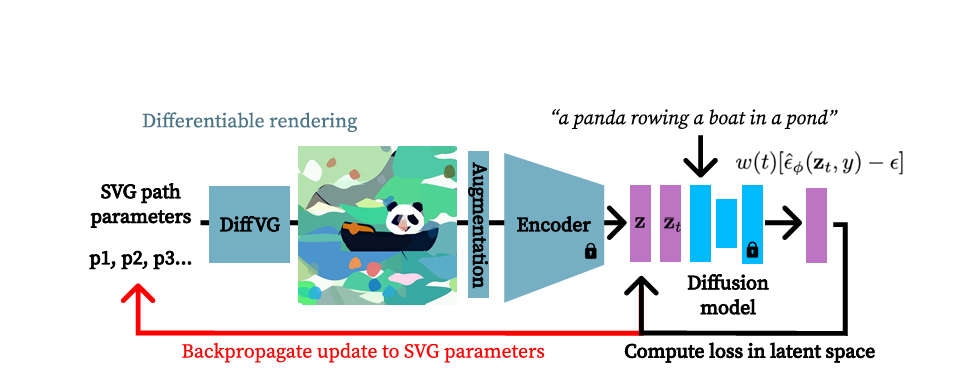
\includegraphics[width=0.85\textwidth]{SDS.png}
\caption{SDS optimization loop in VectorFusion~\cite{jainVectorFusionTexttoSVGAbstracting2022}.}
\label{fig:sds_loop}
\end{figure}


\begin{figure}[htbp]
\centering
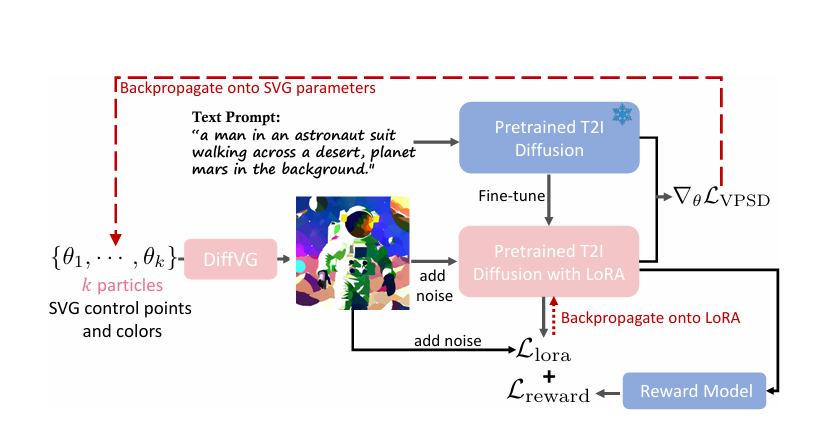
\includegraphics[width=0.85\textwidth]{VPSD!.png}
\caption{VPSD optimization loop in SVGDreamer~\cite{xingSVGDreamerTextGuided2024}.}
\label{fig:svgdreamer_vpsd}
\end{figure}

The two loops look alike, but they differ in what is trained. 
In SDS (Figure~\ref{fig:sds_loop}) everything except the SVG is frozen. 
The render is encoded and noised, the frozen model predicts the noise, 
and the difference between predicted and added noise flows back through 
DiffVG into one SVG. VPSD (Figure~\ref{fig:svgdreamer_vpsd}) keeps the 
diffusion model frozen too, but adds two things.

There are $k$ SVGs (particles) instead of one. A LoRA copy of the diffusion 
model is trained on their renders, and the SVG update comes from the difference 
between the frozen model and this copy. A reward model also scores the particles 
and reweights them. The authors report this gives better-looking results and 
faster convergence~\cite{xingSVGDreamerTextGuided2024}.

\subsection{Neural Implicit Representation}

NIVeL~\cite{thamizharasanNIVeLNeuralImplicit2024} and 
NeuralSVG~\cite{polaczekNeuralSVGImplicitRepresentation2025} take 
a different approach to the same optimization loop. 
They store geometry as the weights of a small MLP, instead of 
storing geometry as explicit B\'{e}zier coordinates that are 
adjusted directly. In NeuralSVG the network takes a shape index 
and outputs the geometry for that shape. In NIVeL it takes a pixel 
coordinate and returns which layer covers it. Nothing is stored as an explicit path.

This brings different properties to optimization-based approaches. In 
parametric methods each path is an independent object, and 
optimization can push the paths in different directions. With an 
MLP, all shapes come from the same learned function, which 
creates a bias toward global coherence. NIVeL uses this to 
decompose scenes into layered components, where each layer is 
a separate neural field whose zero-level set defines a shape 
boundary. NeuralSVG assigns each shape a fixed index 
(Section~\ref{sec:implicit}). The outputs from 
both tend to be cleaner and more organized than purely 
parametric optimization, but they still need a full optimization 
run for every new prompt. Figure~\ref{fig:opt_neural_pipelines} 
compares the two pipelines.

\begin{table}[htbp]
\centering
\caption{Architectural overview of optimization-based 
SVG generation methods. Trainables: what is updated, 
per-instance parameters optimized at inference time, 
except for Im2Vec, whose network weights are trained once. 
Init.: how primitives are placed before optimization. 
Supervision: the loss that drives the update. 
Representation: how geometry is stored while it is optimized.}
\label{tab:arch_optbased}
\footnotesize
\begin{tabularx}{\textwidth}{@{}l l l l X@{}}
\toprule
\textbf{Model} & \textbf{Trainables} & \textbf{Init.} 
& \textbf{Supervision} & \textbf{Representation} \\
\midrule
LIVE         & SVG param.          & Error-driven     
             & Pixel recon.        & Parametric       \\
SAMVG        & SVG param.          & Mask-based       
             & Pixel recon.        & Parametric       \\
Im2Vec       & Encoder + RNN       & Image encoding   
             & Pixel recon.        & Parametric paths \\
VectorFusion & SVG param.          & Random/Trace     
             & SDS                 & Parametric       \\
SVGDreamer   & SVG param. + LoRA   & Attention (SIVE) 
             & VPSD                & Parametric       \\
SVGDreamer++ & SVG param. + LoRA   & Random + HIVE    
             & VPSD + HIVE         & Structured param.\\
NeuralSVG    & MLP weights + LoRA  & Saliency-based   
             & SDS                 & Neural implicit  \\
NIVeL        & MLP weights         & Random weights   
             & SDS                 & Neural implicit  \\
\bottomrule
\end{tabularx}
\end{table}

Table~\ref{tab:arch_optbased} summarizes the 
architectural components of the optimization-based 
methods. For all models here except Im2Vec, 
``Trainables'' means per-instance parameters optimized 
at inference time. None of them needs a training 
dataset. Supervision comes from the input image or from 
a frozen pretrained model. Im2Vec is different. Its 
trainables are network weights, learned once from 
raster images.



\section{Dataset-Driven Methods}
\label{sec:datasetdriven}

Dataset-driven methods learn structural patterns from collections of vector graphics
and generate through a trained forward pass. The
optimization happens during training, not at inference.
Outputs reflect statistical regularities in the training
data rather than the iterative refinement of any single
instance. These methods are more constrained by the training corpus
but can produce more consistent and visually appealing results
without the computational cost of optimization at inference.

DeepSVG~\cite{carlierDeepSVGHierarchicalGenerative2020}
is the foundational model in this family. It learns a
hierarchical latent space over SVG path commands using
a transformer-based encoder-decoder trained on the
SVG-Icons8 dataset.
The latent space separates path-level and command-level
representations, allowing the model to capture both coarse
shape organization and fine geometric detail. At inference,
all SVG commands are decoded from a sampled latent vector
in a single forward pass, not one after another~\cite{carlierDeepSVGHierarchicalGenerative2020}. DeepSVG demonstrated that structured SVG
generation from a learned latent space is feasible, and
also exposed the difficulty of maintaining geometric
validity across long command sequences.

DeepIcon~\cite{bingDeepIconHierarchicalNetwork2024} applies a similar framework
to icon vectorization specifically, trained on the same
SVG-Icons8 dataset of simple icons. The domain-specific training
produces outputs with more consistent style and geometry
than general-purpose models, though generalization beyond
the training distribution is limited by design.

LayerTracer~\cite{songLayerTracerCognitiveAlignedLayered2025} approaches the problem
differently. Rather than predicting SVG commands from a
latent vector, it models the construction process of
vector graphics layer by layer. A diffusion-based
architecture generates intermediate structural
representations that guide each new layer, approximating
the sequential way designers build graphics in practice.
This process-aware formulation produces outputs with more
meaningful layer organization than direct command
prediction, with direct consequences for editability.

T2V-NPR~\cite{zhangTexttoVectorGenerationNeural2024} combines dataset training
with per-prompt optimization. It first trains a neural path VAE
on the FIGR-8-SVG icon dataset, so the latent space learns
what a regular, smooth path looks like. For a new prompt there is
no forward pass. Path latents in this learned space are optimized
with VSD from a pretrained diffusion model, and the result is then
refined with layer-wise vectorization~\cite{zhangTexttoVectorGenerationNeural2024}.
So T2V-NPR is a hybrid: a trained path prior with per-instance
optimization on top. It is described in this section because its
path prior comes from a dataset, but its inference works like
the optimization methods above.

SVGFusion~\cite{xingSVGFusionScalableTexttoSVG2025} is the most architecturally
complex model in this family. It first learns a continuous
latent space of vector graphics using a Vector-Pixel Fusion
Variational Autoencoder (VP-VAE), which encodes each SVG
together with its rendering. Generation
then occurs through a Vector Space Diffusion Transformer
(VS-DiT), which operates entirely in this learned latent
space. This makes SVGFusion distinct from the
semantic-supervised optimization methods in the previous
section: where VectorFusion and SVGDreamer use diffusion
gradients to guide per-instance optimization in pixel space,
SVGFusion uses a diffusion process over a learned vector
distribution to sample new SVGs directly. The outputs
reflect the statistical structure of the training corpus
rather than the convergence of any optimization loop. 
Table~\ref{tab:arch_dataset} summarizes the 
architectural components of the dataset-driven 
methods.

\begin{table}[htbp]
\centering
\caption{Architectural overview of dataset-driven 
SVG generation methods. Training data refers to 
the dataset used for offline model training.}
\label{tab:arch_dataset}
\footnotesize
\begin{tabularx}{\textwidth}{@{}l l l l X@{}}
\toprule
\textbf{Model} & \textbf{Trainables} & \textbf{Data} 
& \textbf{Supervision} & \textbf{Representation} \\
\midrule
DeepSVG      & VAE + Transformer   & SVG-Icons8       
             & Recon. + KL         & Sequential tokens \\
DeepIcon     & Transformer         & SVG-Icons8       
             & Reconstruction      & Sequential tokens \\
SVGFusion    & VP-VAE + VS-DiT     & SVGX             
             & Recon. + Denoising  & Continuous latent \\
T2V-NPR      & NPR-VAE + LoRA      & FIGR-8-SVG       
             & VSD                 & Neural path repr. \\
LayerTracer  & DiT + LoRA          & 20k layered SVGs 
             & Denoising           & Layered sequences \\
\bottomrule
\end{tabularx}
\end{table}

Unlike the optimization-based group, every model here has a 
training corpus. The representation column also shifts 
away from parametric paths toward sequential tokens, latent 
spaces, and layered sequences, reflecting a fundamentally 
different approach to how SVG structure is encoded.



Table~\ref{tab:model_overview} summarizes the thirteen models 
analyzed in this thesis. The \textit{Inference} column 
distinguishes between methods that optimize vector parameters 
at inference time (\textit{Iterative Opt.}) and methods that 
generate SVGs through a single trained forward pass 
(\textit{Forward Dec.}). The \textit{Supervision} column 
indicates the primary signal driving generation: 
\textit{Pixel recon.} refers to reconstruction against a 
target raster image without a pretrained model, \textit{Semantic} to 
signals derived from frozen pretrained models (diffusion or 
CLIP), and \textit{Supervised} to training against 
ground-truth SVG data. \textit{Hybrid} in the Inference 
column marks methods that combine a trained model with a 
per-instance optimization or vectorization step. Task types distinguish between 
\textit{Vectorization} (raster image as input, SVG as 
output), \textit{Text-to-SVG} (text prompt as input), and 
\textit{Unconditional Generation} (no input at inference --- SVG 
sampled directly from a learned latent space).

\begin{table}[htbp]
\centering
\caption{Overview of the thirteen models analyzed in this 
thesis, organized by generation strategy.}
\label{tab:model_overview}
\footnotesize
\begin{tabularx}{\textwidth}{l l l l l X}
\toprule
\textbf{Model} & \textbf{Task} & \textbf{Inference} & 
\textbf{Input} & \textbf{Output} & \textbf{Supervision} \\
\midrule
LIVE         & Vectorization      & Iterative Opt. & Image    & Paths        & Pixel recon. \\
SAMVG        & Vectorization      & Iterative Opt. & Image    & Paths        & Pixel recon. \\
Im2Vec       & Vectorization      & Forward Dec.   & Image    & Paths        & Pixel recon. \\
\midrule
VectorFusion & Text-to-SVG        & Iterative Opt. & Text     & Paths        & Semantic   \\
SVGDreamer   & Text-to-SVG        & Iterative Opt. & Text     & Paths        & Semantic   \\
SVGDreamer++ & Text-to-SVG        & Iterative Opt. & Text     & Paths        & Semantic   \\
NIVeL        & Text-to-SVG        & Iterative Opt. & Text     & Layers/Paths & Semantic   \\
NeuralSVG    & Text-to-SVG        & Iterative Opt. & Text     & Layers/Paths & Semantic   \\
\midrule
DeepSVG      & Unconditional      & Forward Dec.   & None     & Paths        & Supervised \\
DeepIcon     & Vectorization      & Forward Dec.   & Image    & Layers/Paths & Supervised \\
SVGFusion    & Text-to-SVG        & Forward Dec.   & Text     & Layers/Paths & Supervised \\
T2V-NPR      & Text-to-SVG        & Hybrid         & Text     & Layers/Paths & Sup. + Semantic \\
LayerTracer  & Text-to-SVG        & Hybrid         & Text/Img & Layers/Paths & Supervised \\
\bottomrule
\end{tabularx}
\end{table}

The split between Iterative Opt. and Forward Dec. in the 
Inference column maps almost cleanly onto the two families: 
every optimization-based model except Im2Vec refines at 
inference time, while every dataset-driven model except 
T2V-NPR generates through a forward pass. Im2Vec is trained 
and then decodes in a single pass. T2V-NPR trains a path 
prior and then optimizes for each prompt. LayerTracer is 
labeled Hybrid because it combines a trained diffusion model 
with a per-instance vectorization step.


The thirteen models described here differ in representation 
and supervision, and those two dimensions do not operate 
independently. A model's representation constrains what 
supervision signals are meaningful, and the choice of 
supervision often determines which representations are 
practical. The next two chapters trace these interactions: 
first through representation (Chapter~\ref{ch:representation}), 
then through supervision (Chapter~\ref{ch:supervision}).
    \chapter{Vector Representation in SVG Generation}
\label{ch:representation}

How a model represents vector graphics internally during generation is not the same thing as what it outputs. 
The final result is always an SVG file. What differs is the intermediate form where shapes are created,
manipulated, and decoded. The four representation types introduced in Chapter~\ref{ch:Background} each encode the same underlying
geometry differently and that difference affects what the generated SVG looks like when you actually open it.
This chapter works through four representation families as they appear across the chosen models, 
then examines what each one does to the structure of the output. 
Figure~\ref{fig:rocket_grid} shows the differences qualitatively.

\section{Parametric Representations}
\label{sec:parametric}

Parametric representations are the purest form of how SVG already works. Every path is stored as B\'{e}zier control points, 
stroke attributes, and fill colors, the same parameters that appear in the file itself (Section~\ref{sec:parametric_repr}). 
Once DiffVG made rasterization differentiable~\cite{liDifferentiableVectorGraphics2020a} (Section~\ref{sec:diffvg}), 
these parameters became directly optimizable against image-based or semantic objectives. LIVE, SAMVG, VectorFusion, 
and SVGDreamer all build on this foundation~\cite{maLayerwiseImageVectorization2022, zhuSAMVGMultistageImage2023, 
jainVectorFusionTexttoSVGAbstracting2022, xingSVGDreamerTextGuided2024}.
This should make parametric outputs the most editable of any representation. Every shape is an explicit geometric object a designer can select. 
But that breaks down at scale. On complex images, LIVE is run with up to 256 paths, added layer by layer~\cite{maLayerwiseImageVectorization2022}. 
Open that output in Illustrator or Inkscape and the problem is the image looks fine, 
but selecting a single object means clicking through dozens of overlapping fragments that do not correspond to any recognizable component. 
Fine visual detail needs more paths, not more expressive ones, so these methods are run with large path budgets. 
Only LIVE and SVGDreamer++ add paths during optimization~\cite{maLayerwiseImageVectorization2022, xingSVGDreamerAdvancingEditability2025}. 
SVGDreamer++~\cite{xingSVGDreamerAdvancingEditability2025} identifies this path entanglement explicitly as a failure mode of optimization-based parametric methods.
The representation itself is not the problem. Nothing in the optimization process stops paths from piling up, which is the real issue for editability.

Which primitives do these models actually use? DiffVG can render paths, circles, ellipses, rectangles, and 
polygons~\cite{liDifferentiableVectorGraphics2020a}. But most parametric models here use only one of them: closed paths 
made of cubic B\'{e}zier segments. LIVE and VectorFusion use four cubic segments per 
path~\cite{maLayerwiseImageVectorization2022, jainVectorFusionTexttoSVGAbstracting2022}, and Im2Vec decodes every shape 
as a closed B\'{e}zier path~\cite{reddyIm2VecSynthesizingVector2021}. A closed path can look like a circle, but it is never 
stored as one, so the file contains no \texttt{<circle>} or \texttt{<rect>} elements. SVGFusion is the exception. 
It is trained on real SVG files and keeps their circles, rectangles, and ellipses~\cite{xingSVGFusionScalableTexttoSVG2025}.



\section{Sequential Representations}
\label{sec:sequential}

Sequential models produce some of the most compact outputs in the analyzed set. 
Paths are few, shapes are distinct, and the resulting SVG files are small enough to read by hand.
The reason is structural. Sequential representations treat vector graphics as ordered sequences of drawing commands,
mirroring the actual structure of SVG path data. DeepSVG~\cite{carlierDeepSVGHierarchicalGenerative2020} 
extended this formulation to structured SVG icons using a hierarchical VAE with a transformer decoder. 
DeepIcon~\cite{bingDeepIconHierarchicalNetwork2024} follows the same approach for icon vectorization. 
These models generate a series of commands that describe how the graphic is constructed step by step.
The catch is complexity. In models that predict one command after another, such as SketchRNN (Section~\ref{sec:sequential_repr}), 
every additional command increases the chance that prediction errors grow. 
A mistake appearing early in a long sequence can break everything that comes after it. 
DeepSVG avoids this by decoding all commands at once~\cite{carlierDeepSVGHierarchicalGenerative2020}, but it is still limited by its data. 
It trains on SVG-Icons8~\cite{carlierDeepSVGHierarchicalGenerative2020}, 
which consists of simple icons with small path counts and the outputs reflect that constraint.
In general most of the models that are trained on datasets have specific constraints based on dataset characteristics.
DeepSVG fixes the order of commands itself and does not leave it to the model. In preprocessing, rectangles, circles, and 
ellipses become paths. Every icon is scaled to 256 $\times$ 256. Each path then starts at its topmost-leftmost point 
and runs clockwise. In the ordered variant of the loss, the paths 
themselves are sorted lexicographically by their start position~\cite{carlierDeepSVGHierarchicalGenerative2020}. 
So the same icon always gives the same sequence, and the model learns one order instead of all possible ones.
There is also a more fundamental limitation: a procedural command sequence does not encode explicit spatial hierarchy. 
The model generates commands in order but nothing in the representation directly tells you which commands belong to which semantic region.


\section{Implicit Neural Representations}
\label{sec:implicit}

NeuralSVG~\cite{polaczekNeuralSVGImplicitRepresentation2025} represents each SVG as a set of shape indices, 
where each index corresponds to a single shape. A small MLP learns to map these indices to B\'{e}zier control points and fill colors. 
So the representation is the network weights and the geometry only exists when you query the network for it.
This is fundamentally different from storing control points or commands explicitly. 
The model maintains stable shape correspondence during training, meaning each index always maps to the same visual region, 
which prevents inconsistent outputs across iterations. 

NIVeL~\cite{thamizharasanNIVeLNeuralImplicit2024} follows a similar approach, 
encoding the entire layered structure implicitly where each layer is defined by a continuous neural function over the image domain.
The outputs from both models tend to look globally coherent. Layers are clean and shapes do not bleed into each other. 
NeuralSVG produces compositions that hold together in ways that purely parametric outputs with hundreds 
of paths often do not and doing it with just 16 shapes (Figure~\ref{fig:supervision_comparison}). The cost is that individual shapes are not directly accessible until the network output is 
converted into discrete primitives. How clean that conversion is determines whether the final SVG is practically editable.

\section{Latent Space as a Generative Layer}
\label{sec:latent}

As established in Section~\ref{sec:latent_repr}, a latent space is not a geometric representation but a generative layer 
that sits on top of one. The geometry is always produced by a decoder that translates latent vectors back into parametric paths 
or sequential commands. What the latent space contributes is compression, many graphics are mapped into a shared numerical embedding 
learned during training. DeepSVG applies this by encoding path command sequences into latent vectors and training a transformer 
decoder to reconstruct them~\cite{carlierDeepSVGHierarchicalGenerative2020}, building on the VAE framework (Section~\ref{sec:latent_repr}). 
The latent space captures structural regularities across the training dataset, so new SVGs can be generated by sampling from this space.

SVGFusion~\cite{xingSVGFusionScalableTexttoSVG2025} extends this idea by running a diffusion process entirely within the learned latent 
space of a pretrained vector encoder. T2V-NPR takes a different route, arguing that global SVG-level 
latent spaces are too constrained for diverse path combinations and instead learns a neural path representation at the individual 
path level~\cite{zhangTexttoVectorGenerationNeural2024}.

\section{Representation Boundaries in Practice}
\label{sec:rep_boundaries}

Most models do not stay cleanly inside one representation family. VectorFusion and SVGDreamer optimize parametric
primitives directly while using a latent diffusion model as the semantic prior. The parametric layer provides geometric 
interpretability, while the latent model provides the semantic coherence that pure geometric optimization cannot achieve alone.

NeuralSVG imposes an order on its shapes with a dropout-based regularization: during training, the shape sequence 
is randomly cut off, so the first shapes have to carry the coarse structure of the scene on their 
own~\cite{polaczekNeuralSVGImplicitRepresentation2025}. Together with the fixed index mapping 
(Section~\ref{sec:implicit}), this makes individual shapes separable. 
LayerTracer~\cite{songLayerTracerCognitiveAlignedLayered2025} crosses a different boundary: its training data is sequential 
(step-by-step construction sequences built from about 20,000 layered SVGs made by designers), but the output is a layered parametric SVG where each layer 
corresponds to a meaningful visual component. The model learns layer separation as a structural convention from how designers 
actually build graphics. These combinations exist because no single 
representation handles visual realism and structural clarity at the same time.

\section{Representation, Editability, and Structural Outcomes}
\label{sec:rep_editability}

Open any SVG in Illustrator or Figma and you expect to click on a shape and move it. That is the whole point.
Whether an AI-generated SVG actually supports that depends more on how the model represents geometry internally 
than on how the rendered output looks.

The four rockets in Figure~\ref{fig:rocket_grid} show what this means concretely. 
DeepSVG works with monochrome icons like this rocket, with around 15 to 30 paths. 
The rocket in the figure is a sample from the SVG-Icons8 dataset, not a generated output, 
but it shows the kind of output DeepSVG is trained to produce. 
It stays at the level of an icon, not a photorealistic scene, because it is trained on 
simple icons with few paths (Section~\ref{sec:sequential}). 
A designer could open that file and rearrange things. SVGDreamer generates the same 
subject using 256 to 512 optimized B\'{e}zier paths~\cite{xingSVGDreamerTextGuided2024}. 
Visually rich but structurally opaque, most of those paths overlap without corresponding 
to any recognizable component. NeuralSVG renders its rocket with exactly 16 shapes, 
each mapped through an MLP~\cite{polaczekNeuralSVGImplicitRepresentation2025}. 
In the figure these read as a few large regions: a dark body with a lighter stripe, 
angled fins, a pale flame at the tail, and the flat background. 
That is roughly a 30x reduction in element count. SVGFusion does not sit in between. 
Its rocket is built from only a handful of filled shapes, so in element count it is closer 
to DeepSVG than to SVGDreamer. What differs is the vocabulary: SVGFusion can output 
B\'{e}zier paths but also circles, rectangles, and 
ellipses~\cite{xingSVGFusionScalableTexttoSVG2025}, 
because its latent space was trained on real SVG files that use these elements.
Table~\ref{tab:rep_structure} summarizes these counts.

\begin{figure}[htbp]
    \centering
    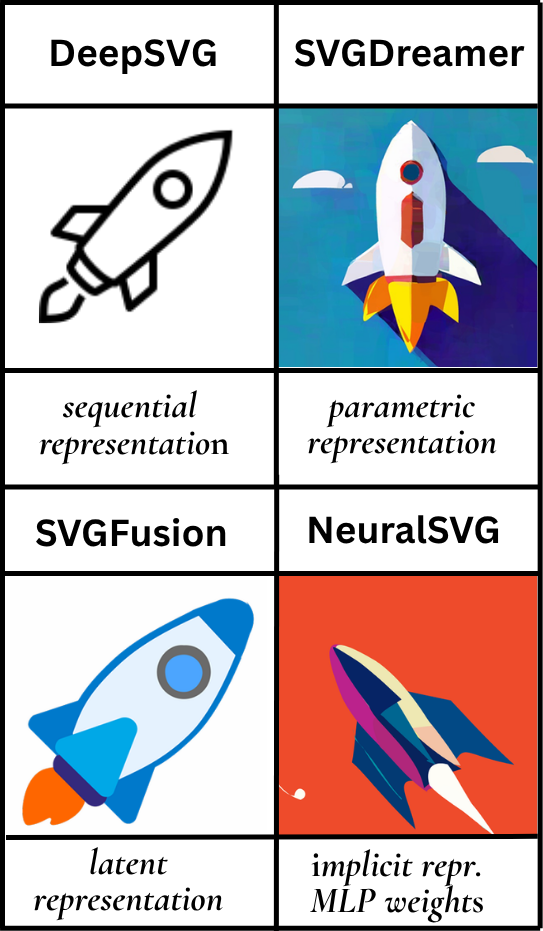
\includegraphics[width=0.42\textwidth]{representation.png}
    \caption{Rockets illustrating the three geometric representations 
    and the latent generative layer. Top left: a rocket icon from the SVG-Icons8 
    dataset that DeepSVG (sequential) is trained 
    on~\cite{carlierDeepSVGHierarchicalGenerative2020}; this 
    is a dataset sample, not a DeepSVG output. The other three 
    are generated outputs. Top 
    right: SVGDreamer (parametric). Bottom left: SVGFusion 
    (latent space as a generative layer; the SVG it decodes is parametric). Bottom right: NeuralSVG (implicit neural). The 
    SVGDreamer and SVGFusion outputs are reproduced 
    from~\cite{xingSVGFusionScalableTexttoSVG2025}, the NeuralSVG 
    output 
    from~\cite{polaczekNeuralSVGImplicitRepresentation2025}.}
    \label{fig:rocket_grid}
\end{figure}

\begin{table}[htbp]
\centering
\caption{Structural consequences of representation choice. The latent row is a generative layer on top of a geometric representation, not a geometric representation itself. Path counts reflect default configurations reported in the respective papers; n.r.\ = not reported.}
\label{tab:rep_structure}
\begin{tabular}{l l l p{5.6cm}}
\hline
\textbf{Representation} & \textbf{Path Counts} & \textbf{Editability} & \textbf{Typical Output} \\
\hline
Parametric      & 64--512   & Low    & Visually rich, paths overlap heavily \\
Sequential      & 15--30    & Medium & Clean icons, breaks on complex scenes \\
Implicit neural & 16 (fixed)& High   & Few shapes, each semantically meaningful \\
Latent          & Few (n.r.) & Medium & Uses full SVG vocab, looks designed \\
\hline
\end{tabular}
\end{table}

The number of shapes a model produces matters more for practical editability. 
Parametric representations should be the most editable since every shape is an explicit geometric object. 
But that advantage vanishes when the path count gets into the hundreds. 
Sequential and latent representations produce compact output within bounded domains. 
Implicit representations give the cleanest decomposition but at a computational cost.

What actually drives clean structure is not the representation itself but what constraints are placed on it. 
Methods that use segmentation masks to initialize primitives (SAMVG)~\cite{zhuSAMVGMultistageImage2023}, 
saliency maps to place shapes (NeuralSVG)~\cite{polaczekNeuralSVGImplicitRepresentation2025}, or 
construction-sequence training data (LayerTracer)~\cite{songLayerTracerCognitiveAlignedLayered2025} 
all produce cleaner boundaries regardless of their underlying representation type. 
Representation defines what kinds of structures are possible. 
Initialization and supervision determine whether useful structure actually shows up in the output.

\section{Summary}
\label{sec:rep_summary}

Representation sets the boundaries for what a model can produce. 
What it actually produces depends on supervision. 
The next chapter looks at how different supervision
signals push the geometry in different directions.

    \chapter{Supervision and Guidance Strategies for SVG Generation}
\label{ch:supervision}

Representation defines how vector graphics are encoded during generation. 
Supervision determines what happens to those representations during training or optimization.
In SVG generation, the supervision signal is whatever tells the model whether its current output 
is getting closer to the goal or further away. That signal might come from a target image, 
a text prompt scored by CLIP, a diffusion model's learned prior, or the structure of a training dataset itself.

What makes supervision in this domain unusual is that it interacts with representation. 
A similar loss applied to explicit B\'{e}zier paths and to implicit neural fields 
produces different geometric outcomes. The representation is not the only difference between such models, 
but it is the biggest one (Section~\ref{sec:rep_sup_interaction}). 
This is why Chapters~\ref{ch:representation} and~\ref{ch:supervision} need to be read together, 
neither dimension explains the structural properties of the output on its own.

Table~\ref{tab:supervision_overview} provides a complete overview of which signal each model uses and when it is applied.

\begin{table}[htbp]
\centering
\caption{Supervision signals used by each of the thirteen models 
analyzed in this thesis.}
\label{tab:supervision_overview}
\begin{tabular}{l l l}
\hline
\textbf{Model} & \textbf{Supervision Signal} & \textbf{Applied} \\
\hline
LIVE & UDF pixel loss + Xing loss & Inference \\
SAMVG & MSE + LPIPS + SAM segmentation init & Inference \\
Im2Vec & L2 via differentiable rendering & Training \\
VectorFusion & SDS from Stable Diffusion & Inference \\
SVGDreamer & VPSD from Stable Diffusion & Inference \\
SVGDreamer++ & VPSD + HIVE masks + reward model & Inference \\
NeuralSVG & SDS + fine-tuned LoRA adapter & Inference \\
NIVeL & SDS from DeepFloyd & Inference \\
DeepSVG & Cross-entropy + L1 + KL divergence & Training \\
DeepIcon & Cross-entropy + CLIP embedding & Training \\
SVGFusion & KL + latent-space denoising (VS-DiT) & Training \\
T2V-NPR & VSD + neural path VAE & Both \\
LayerTracer & Denoising on layered construction sequences & Training \\
\hline
\end{tabular}
\end{table}


\section{Reconstruction-Based Supervision}
\label{sec:recon_supervision}

In short: render the SVG, compare it to a target image, update the parameters. 
That is the entire loop. Reconstruction-based supervision is the most 
direct application of the losses described in Section~\ref{sec:recon_losses}, 
and for the optimization methods and Im2Vec it works through DiffVG~\cite{liDifferentiableVectorGraphics2020a}.
Because the target is known, gradients provide clear information about what should change. 
When datasets contain clean SVG examples, models trained this way can absorb typical path 
counts from the data. DeepSVG, DeepIcon, and Im2Vec all use reconstruction 
objectives~\cite{carlierDeepSVGHierarchicalGenerative2020, bingDeepIconHierarchicalNetwork2024, reddyIm2VecSynthesizingVector2021}, 
each with a different combination of losses (Table~\ref{tab:supervision_overview}). 
DeepSVG and DeepIcon compare their predictions against ground-truth SVG commands. 
Im2Vec has no SVG targets at all: it is trained on raster images, and its reconstruction loss 
compares the rendered output with the input image through differentiable rendering. 
Once trained, generation is a single forward pass with no further optimization (Chapter~\ref{ch:Landscape}).

The structural quality of the output comes from the dataset, not from the loss. 
The loss only measures visual similarity. A model trained on messy SVGs with redundant 
paths would learn to reproduce that mess. A model can achieve low 
reconstruction error while producing overlapping geometry, 
because pixel-level matching does not care about what the SVG file looks like on the inside. 
Reconstruction supervision also requires a reference image, so it cannot support text-to-SVG generation on its own.


\section{Semantic Guidance with Vision--Language Models}
\label{sec:clip_guidance}

CLIP-based guidance (Section~\ref{sec:clip}) can score how well a rendered SVG matches a text prompt, when no reference image exists. 
This makes open-ended generation possible without paired SVG datasets.
CLIP measures alignment in embedding space, not structural correctness. 
Optimization can introduce extra primitives to push the embedding score higher, 
and there is nothing in the signal that penalizes fragmented output. 
In practice, CLIP guidance is rarely used alone. In VectorFusion~\cite{jainVectorFusionTexttoSVGAbstracting2022}, 
CLIP only ranks raster samples from the diffusion model before they are traced, 
and the optimization itself runs on SDS.


\section{Diffusion-Based Supervision}
\label{sec:diffusion_supervision}

Diffusion-based supervision has become the dominant strategy for text-to-SVG generation. 
These methods use a pretrained diffusion model as a perceptual prior, instead of relying on reference images, the same as CLIP. 
The diffusion model has already learned what images should look like. 
The SVG parameters get adjusted until the diffusion model thinks the rendered output looks right for the given text prompt.

The mechanism is Score Distillation Sampling (SDS). Variational Score Distillation (VSD) 
was introduced by ProlificDreamer~\cite{wangProlificDreamerHighFidelityDiverse2023} to address the oversaturation 
that standard SDS tends to produce, and SVGDreamer~\cite{xingSVGDreamerTextGuided2024} builds its VPSD on it. 
Both are described in Section~\ref{sec:sds_vsd}. 
What matters for this chapter is what each variant does to the geometry.

VectorFusion and NIVeL use standard SDS~\cite{jainVectorFusionTexttoSVGAbstracting2022, thamizharasanNIVeLNeuralImplicit2024}. 
VectorFusion takes it from Stable Diffusion. NIVeL takes it from DeepFloyd, which denoises in pixel space, so no image encoder sits in the loop~\cite{thamizharasanNIVeLNeuralImplicit2024}. 
NeuralSVG adds a fine-tuned LoRA adapter on top of SDS~\cite{polaczekNeuralSVGImplicitRepresentation2025}. 
SVGDreamer replaces SDS entirely with VPSD~\cite{xingSVGDreamerTextGuided2024}. 
Figure~\ref{fig:supervision_comparison} shows the outputs side by side from the same prompt. 
VectorFusion produces over-smoothed geometry with 64 shapes. 
SVGDreamer improves diversity but uses 256 shapes to get there. 
NeuralSVG reaches comparable visual quality with 16 shapes. 

Diffusion gradients operate in pixel space and reward perceptual realism. 
They do not reward geometric simplicity. Without structural constraints, 
these methods need a large path budget to satisfy visual objectives.
Inference cost is also high, every generation requires repeated rendering and 
diffusion evaluation cycles, unlike dataset-driven models that produce output in a single pass.

\begin{figure}[htbp]
    \centering
    \begin{tabular}{ccc}
    \textbf{VectorFusion} & \textbf{SVGDreamer} & \textbf{NeuralSVG} \\
    \small{SDS} & \small{VPSD} & 
    \small{SDS + LoRA} \\[4pt]
    
\includegraphics[width=0.25\textwidth]{vectorfusion_img.png} &
    
\includegraphics[width=0.25\textwidth]{svgdreamer256_img.png} &
    
\includegraphics[width=0.25\textwidth]{neuralsvg16_img.png} \\
    \end{tabular}
    \caption{Three diffusion-based supervision variants generating 
    from the same prompt. VectorFusion (SDS, 64 shapes) produces 
    over-smoothed geometry. SVGDreamer (VPSD, 256 shapes) improves 
    diversity but uses four times as many primitives. NeuralSVG 
    (SDS with LoRA, 16 shapes) achieves comparable visual quality 
    with the fewest shapes. Images reproduced 
    from~\cite{xingSVGFusionScalableTexttoSVG2025, 
    polaczekNeuralSVGImplicitRepresentation2025}.}
    \label{fig:supervision_comparison}
\end{figure}


\section{Dataset Supervision vs.\ Per-Instance Supervision}
\label{sec:dataset_vs_instance}

When supervision is applied changes what kind of output you get.
Dataset-supervised models learn from collections of SVG graphics during training. 
DeepSVG~\cite{carlierDeepSVGHierarchicalGenerative2020} and DeepIcon~\cite{bingDeepIconHierarchicalNetwork2024} 
are trained on reconstruction objectives against SVG data. Im2Vec~\cite{reddyIm2VecSynthesizingVector2021} 
is trained on raster images instead, with reconstruction through differentiable rendering. 
Once trained, generation requires no further optimization for any of the three. LayerTracer~\cite{songLayerTracerCognitiveAlignedLayered2025} 
takes this further: it trains on construction sequences derived from about 20,000 layered SVGs made by designers. 
Each graphic is rebuilt in a deliberate layer order that mimics how designers actually build graphics (Figure~\ref{fig:serpentine}). 
The dataset structure itself is the supervision prior. The model learns to produce layered outputs not because a loss function rewards 
layering, but because every training example was built that way.

\begin{figure}[htbp]
    \centering
    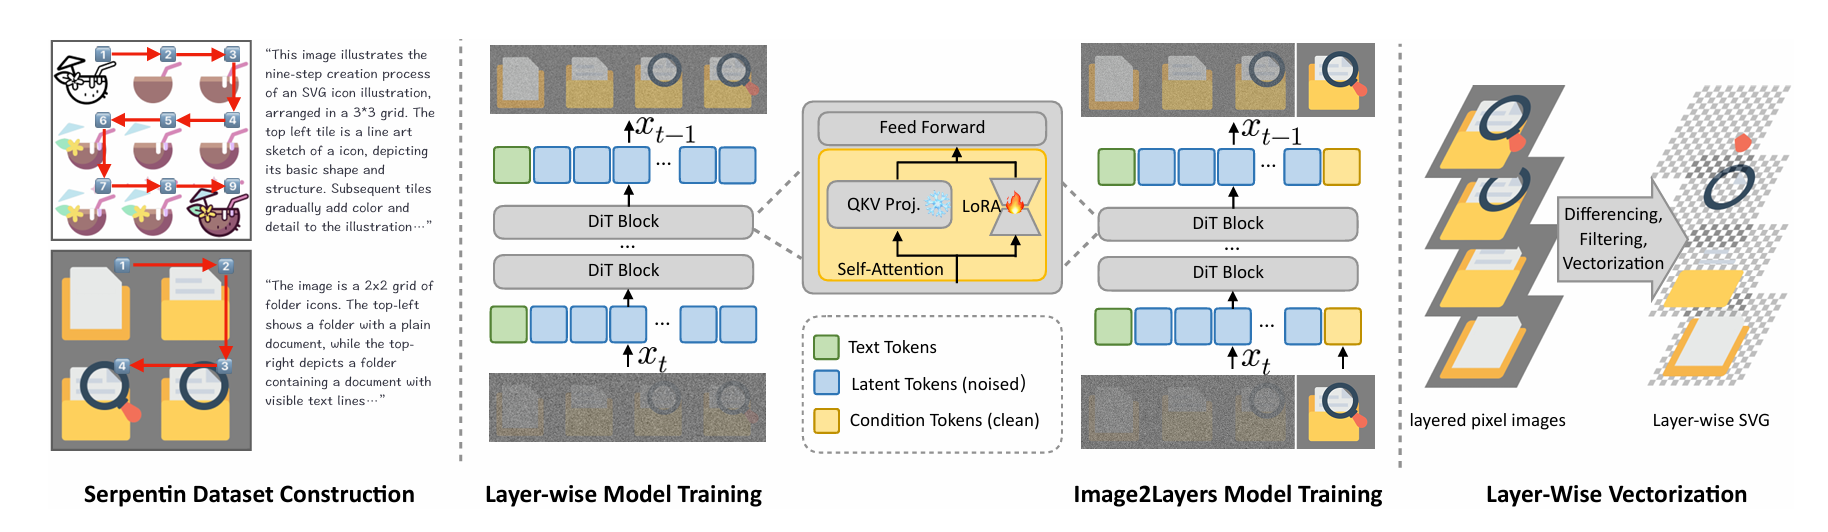
\includegraphics[width=0.85\textwidth]{latertracer trng.png}
    \caption{Step-by-step construction sequence from the training 
    data of LayerTracer~\cite{songLayerTracerCognitiveAlignedLayered2025}. 
    The frames are arranged in a serpentine grid layout, so 
    consecutive steps sit next to each other. 
    Each stage adds a new layer, mimicking how a designer would 
    build the graphic incrementally. The dataset structure itself 
    encodes the supervision prior.}
    \label{fig:serpentine}
\end{figure}

Per-instance supervision works on a completely different timescale. 
LIVE~\cite{maLayerwiseImageVectorization2022}, SAMVG~\cite{zhuSAMVGMultistageImage2023}, 
VectorFusion~\cite{jainVectorFusionTexttoSVGAbstracting2022}, SVGDreamer~\cite{xingSVGDreamerTextGuided2024}, 
NeuralSVG~\cite{polaczekNeuralSVGImplicitRepresentation2025}, and NIVeL~\cite{thamizharasanNIVeLNeuralImplicit2024} all optimize vector parameters from scratch for each input. 
No model is trained. Structure changes dynamically in response to each prompt or image, 
which is flexible but computationally expensive.
T2V-NPR~\cite{zhangTexttoVectorGenerationNeural2024} combines both: it learns a path latent space 
from a dataset during training and then optimizes path latents for each prompt at inference. 
SVGFusion~\cite{xingSVGFusionScalableTexttoSVG2025} also learns its latent space from data, 
but it does not optimize at inference. It samples new SVGs with its latent diffusion transformer, 
which takes 24 to 36 seconds per SVG. 






\section{Initialization and Structural Priors}
\label{sec:init_priors}

Where optimization starts matters as much as what it optimizes for.
SAMVG~\cite{zhuSAMVGMultistageImage2023} is the clearest example. 
It uses the Segment Anything Model to define semantically meaningful 
regions before any vector optimization begins. The loss function is still pixel reconstruction, 
same as LIVE. But SAMVG's outputs have cleaner boundaries and less path fragmentation, 
because the starting point already encodes where objects are. The kind of supervision did not change. 
The initialization did, and that made the structural difference (Figure~\ref{fig:init_comparison}). 
The two outputs look almost identical at first sight, 
and most people would not notice a difference. But look 
more carefully: SAMVG's output (right) has cleaner shape 
boundaries with fewer overlapping paths, while LIVE's 
output (left) captures finer shading and color transitions 
through denser path layering. The visual fidelity is 
slightly higher in LIVE, but that fidelity comes from 
path fragmentation that makes the file harder to edit.

\begin{figure}[htbp]
    \centering
    \begin{tabular}{cc}
    \textbf{LIVE} & \textbf{SAMVG} \\
    \textbf{Error-driven init} & \textbf{SAM segmentation init} \\[4pt]
    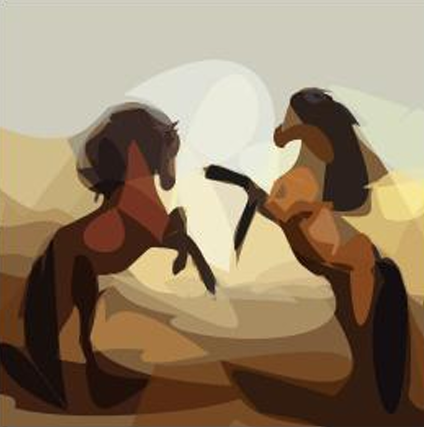
\includegraphics[width=0.36\textwidth]{live_img.png} &
    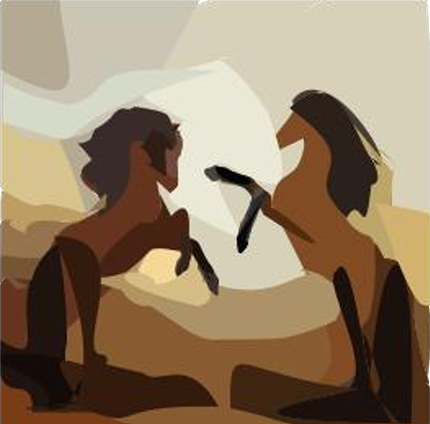
\includegraphics[width=0.36\textwidth]{sam_img.png} \\
    \end{tabular}
    \caption{Both models use pixel reconstruction loss via 
    differentiable rasterization. LIVE adds each new path where 
    the reconstruction error is largest and produces a visually closer match to the target through dense 
    overlapping paths, but the resulting file is fragmented and 
    difficult to edit. SAMVG initializes from segmentation masks 
    and produces cleaner object boundaries with fewer paths, at 
    the cost of reduced visual 
    fidelity~\cite{zhuSAMVGMultistageImage2023}.}
    \label{fig:init_comparison}
\end{figure}

T2V-NPR starts optimization inside a latent space shaped by prior training, 
so even a random starting latent decodes to a regular path. SVGFusion does not optimize at all, 
its structure comes from the training data through sampling. LayerTracer takes the idea further, 
its training data encodes construction order (Figure~\ref{fig:serpentine}), 
so the model learns to produce layered outputs without any explicit structural loss. 
The dataset itself is the structural prior.
When meaningful priors are absent, 
diffusion optimization needs many primitives. When structured initialization is present, 
the same loss produces cleaner geometry with fewer paths. Supervision tells you what the model optimizes for. 
Initialization tells you where it starts. That starting point often determines whether the result is editable.


\section{Summary}
\label{sec:supervision_summary}

Visual quality always comes first.
Clean structure, when it shows up, is a side effect. 
Some models get closer to editability through their training data or initialization, 
but none of the thirteen directly optimizes for it.


    \chapter{Evaluation of SVG Generation}
\label{ch:Evaluation}

Chapter~\ref{ch:supervision} ended with the observation that visual quality 
always comes first. This chapter asks whether evaluation measures anything else.
Evaluating SVG generation is harder than evaluating raster 
image generation. A raster image is just pixels, the only thing that matters is how it looks.
An SVG is a structured artifact 
that has to look right (semantic alignment), be geometrically stable, and remain 
editable. These three requirements do not always point in 
the same direction, and the metrics most commonly used in 
the literature only measure the first one. 
This chapter examines how the thirteen models are evaluated, which metrics are used, where those practices 
fall short, and what a more complete framework would need 
to include.

\section{Evaluation Metrics in Current Practice}
\label{sec:current_eval}

The majority of SVG generation papers evaluate their outputs 
using metrics borrowed directly from raster image generation 
research. The most common are Fréchet Inception Distance 
(FID)~\cite{heuselGANsTrainedTwo2017}, CLIP-based similarity 
scores~\cite{radfordLearningTransferableVisual2021}, 
perceptual similarity measures such as 
LPIPS~\cite{zhangUnreasonableEffectivenessDeep2018}, 
pixel-level reconstruction metrics such as MSE.
All of these share one property: they 
operate on rasterized outputs. The SVG file itself, its 
path structure, is invisible to every one of them.

FID measures the statistical distance between 
distributions of generated and reference images in a feature 
space derived from a pretrained Inception 
network~\cite{szegedy2016rethinking}. In SVG generation, outputs 
are rasterized before computing FID, which means the metric 
captures rendered appearance only. FID also has documented 
technical sensitivities: it is unstable at sample sizes below 
10,000~\cite{heuselGANsTrainedTwo2017}, and scores shift 
significantly depending on the reference distribution. When 
models are evaluated against datasets that overlap with their 
training data, scores appear artificially favorable. Several papers 
in SVG generation still compute it on substantially 
smaller test sets, which makes cross-paper comparison unreliable.

CLIP score measures semantic alignment between a rendered 
image and a text 
prompt~\cite{radfordLearningTransferableVisual2021}. It is useful for 
text-to-SVG tasks where the goal is semantic correctness, 
but like FID it operates entirely in pixel-space. A model 
can achieve strong CLIP scores while producing structurally 
fragmented or completely uneditable SVG output.

LPIPS is a perceptual similarity metric that 
computes feature-based distances using a pretrained 
network~\cite{zhangUnreasonableEffectivenessDeep2018}. 
It correlates better with human perceptual judgments than 
MSE and is used in vectorization tasks where reconstruction 
fidelity against a reference image matters. SAMVG uses LPIPS 
as part of its optimization 
loss~\cite{zhuSAMVGMultistageImage2023}, and it appears as 
an evaluation metric too. The 
limitation is the same, it measures rendered appearance, 
not vector structure.

Mean squared error (MSE) measures pixel-level difference between
rendered output and reference image. LIVE explicitly avoids it as 
a training loss because it produces blurry, color-averaged 
outputs~\cite{maLayerwiseImageVectorization2022}, yet several
papers still use it for comparability.

Human evaluation remains the most practically 
meaningful signal, but also the hardest to standardize. 
Papers typically show qualitative examples or run 
small user studies asking participants to rate realism, 
prompt alignment, or preference. These assessments capture 
properties that numerical metrics miss, but they are 
subjective and rarely reported 
with enough methodological detail to understand the ratings.

Table~\ref{tab:metrics_used} maps which evaluation metrics
each of the thirteen models actually reports. The 
pattern is clear, FID and CLIP dominate text-to-SVG models, 
MSE and LPIPS appear in vectorization models, and structural 
metrics are almost entirely absent across both groups. 
Human evaluation is present in roughly half the papers.


\begin{table}[htbp]
\centering
\caption{Evaluation signals reported across the thirteen 
models. \checkmark\,= reported, \text{--} = not reported.}
\label{tab:metrics_used}
\small
\begin{tabularx}{\textwidth}{l c c c c c c}
\toprule
\textbf{Model} & \textbf{FID} & \textbf{CLIP} & 
\textbf{LPIPS} & \textbf{MSE} & \textbf{User} & 
\textbf{Chamfer} \\
\midrule
LIVE         & --         & --         & --         
             & \checkmark & \checkmark & --         \\
SAMVG        & \checkmark & --         & \checkmark 
             & \checkmark & --         & --         \\
Im2Vec       & --         & --         & --         
             & \checkmark & --         & --         \\
VectorFusion & --         & \checkmark & --         
             & --         & \checkmark & --         \\
SVGDreamer   & \checkmark & \checkmark & --         
             & --         & \checkmark & --         \\
SVGDreamer++ & \checkmark & \checkmark & --         
             & --         & \checkmark & --         \\
NIVeL        & --         & \checkmark & --         
             & --         & --         & --         \\
NeuralSVG    & --         & \checkmark & --         
             & --         & --         & --         \\
DeepSVG      & --         & --         & --         
             & \checkmark & \checkmark & --         \\
DeepIcon     & --         & --         & --         
             & --         & --         & \checkmark \\
SVGFusion    & \checkmark & \checkmark & --         
             & --         & \checkmark & --         \\
T2V-NPR      & \checkmark & \checkmark & --         
             & --         & \checkmark & --         \\
LayerTracer  & \checkmark & \checkmark & --         
             & \checkmark & --         & --         \\
\bottomrule
\end{tabularx}
\end{table}

Three observations follow from this table. First, no model 
reports layer quality as a quantitative metric, despite 
LayerTracer, NeuralSVG, and T2V-NPR all explicitly claiming 
layered outputs as a contribution. Second, T2V-NPR is the 
only model that evaluates geometric smoothness and it 
does so precisely because smoothness is central to its 
architectural claim, not because it is a standard metric 
in the field. Third, DeepIcon is the only model that reports contour-based 
metrics (Chamfer 
Distance)~\cite{bingDeepIconHierarchicalNetwork2024}, which 
measure shape overlap rather than pixel similarity. No other 
model uses these. This pattern suggests that models tend to 
report metrics that favor their specific contributions while 
structural properties remain unmeasured. 
Some benchmarks have begun to recognize this gap. 
SVGEditBench~\cite{nishinaSVGEditBenchBenchmarkDataset2024} 
and SVGEditBench 
V2~\cite{nishinaSVGEditBenchV22025} introduce structured 
editing tasks and evaluate outputs using raster-based, 
contour-based, and description-based metrics including MSE, 
LPIPS, and CLIP text embeddings. SVGenius~\cite{chenSVGenius2025} 
proposes 18 metrics across understanding, editing, and 
generation dimensions. However, both benchmarks are 
designed primarily for LLM-based SVG processing, and 
neither addresses the structural properties of 
optimization-based or dataset-driven generation methods. 
Zhu et al.~\cite{zhuStructuralEvaluationMetrics2026} go further 
and measure structure directly: they remove one element at a time and score each 
element by how much the render changes. 



\section{Evaluation Gaps}
\label{sec:eval_gaps}

The metrics in Table~\ref{tab:metrics_used} share a 
fundamental limitation: none of them require parsing 
the SVG file. They measure what the output looks like 
after rasterization, not what it is made of. This means 
they cannot detect redundant paths, fragmented geometry, 
missing hierarchy, self-intersecting curves, or 
uneditable structure. For vector graphics, these are 
not secondary properties.

\subsection{Structural Redundancy}
Optimization-based 
methods routinely produce outputs where many small 
overlapping paths approximate a region that a designer 
would represent with one or two shapes. LIVE and 
VectorFusion both exhibit this 
behavior~\cite{maLayerwiseImageVectorization2022, 
jainVectorFusionTexttoSVGAbstracting2022}. The SVG renders 
correctly but is structurally opaque. No metric in 
Table~\ref{tab:metrics_used} would detect the difference. 
NeuralSVG achieves a CLIP text-image similarity of 26.94 
using 16 shapes, while VectorFusion reaches 26.33 with 64 
shapes and SVGDreamer 26.58 with 
256~\cite{polaczekNeuralSVGImplicitRepresentation2025}. 
A 16x difference in path count produces near-identical 
scores on the metric most commonly used to evaluate 
these models.

\subsection{Geometric Quality}
Curved paths in 
optimization outputs are sometimes jagged, 
self-intersecting, or discontinuous under zoom. T2V-NPR 
explicitly measures smoothness and its ablation study 
shows that removing the neural path representation drops 
smoothness from 0.80 to 0.53~\cite{zhangTexttoVectorGenerationNeural2024}. 
That is a large structural difference that FID would not 
detect. LIVE introduces a self-intersection penalty 
(Xing loss) during 
optimization~\cite{maLayerwiseImageVectorization2022}, 
but does not report intersection counts as an evaluation 
metric. The gap between what models optimize for 
geometrically and what they report is notable.


\subsection{Editability}
This is the most practically 
important gap. The practical requirement behind this thesis 
(Section~\ref{sec:motivation}) is that generated SVGs 
must be editable by designers in standard tools. 
None of the metrics in Table~\ref{tab:metrics_used} 
measure this. Editability is occasionally demonstrated 
by showing that a generated element can be recolored 
or moved, but this is not systematically evaluated 
across models and no paper defines criteria for what 
counts as editable. 
Human-designed SVGs already exhibit the structural clarity 
that generated outputs lack. 
Figure~\ref{fig:editability_gap} shows a typical example: 
an icon from SVGRepo opened in Inkscape, where every 
shape can be independently selected and modified. The gap 
between what manual design delivers and what generation 
models are evaluated on is part of the problem: editability 
is a practical requirement that the field has not yet 
learned to measure.

\begin{figure}[htbp]
    \centering
    \begin{tabular}{cc}
    
\includegraphics[width=0.4\textwidth]{2.png} &
    
\includegraphics[width=0.4\textwidth]{3.png} \\
    \small{(a) Assembled} & \small{(b) Shapes separated} \\
    \end{tabular}
    \caption{A human-designed SVG icon from SVGRepo, opened 
    and decomposed in Inkscape. The graphic consists of 8 
    B\'{e}zier paths, each representing a distinct visual 
    component: pole, flag body, skull, eyes, and nose. 
    Every shape can be independently selected, moved, 
    recolored, or deleted. This structural clarity is what 
    current evaluation metrics do not capture.}
    \label{fig:editability_gap}
\end{figure}

\section{Efficiency and Reproducibility}
\label{sec:efficiency}

Inference speed and reproducibility are not peripheral 
concerns for SVG generation, they directly determine 
whether a method can be used in practice. 
Table~\ref{tab:reproducibility} summarizes code 
availability, hardware requirements, and inference time 
across all thirteen models.

The efficiency gap between optimization-based and 
dataset-driven methods is worth considering. LIVE, the 
simplest reconstruction-supervised method, requires 
between 2,600 and 10,000 seconds per image on an RTX 
3090 depending on path count~\cite{maLayerwiseImageVectorization2022}. 
VectorFusion takes 10 to 20 minutes per 
SVG~\cite{jainVectorFusionTexttoSVGAbstracting2022}. 
SVGDreamer and SVGDreamer++ require 7 to 14 minutes 
and at least 31GB of VRAM, placing them out of reach 
for standard consumer 
hardware~\cite{xingSVGDreamerTextGuided2024,xingSVGDreamerAdvancingEditability2025}. 
By contrast, LayerTracer generates a layered SVG in 27 
to 34 seconds~\cite{songLayerTracerCognitiveAlignedLayered2025}, 
and SVGFusion in 24 to 36 
seconds~\cite{xingSVGFusionScalableTexttoSVG2025}. These differences are not small. 
Optimization-based methods take minutes to hours because they refine parameters iteratively at inference time.
Dataset-driven models do it in seconds through a single forward pass.

Hardware requirements follow the same pattern but with 
an important exception. Dataset-driven models are faster, 
but several require enterprise-grade infrastructure during 
training, for example, SVGFusion trains on multiple A800 GPUs, and 
LayerTracer on a single A100 with 80GB VRAM. Once trained, 
these models can run inference on less demanding hardware, 
but the training cost creates a barrier for independent 
replication of these models.

Reproducibility is a separate and equally important 
concern for those who want to replicate the work.
Code availability was recorded for every model but was not 
a selection criterion (Section~\ref{sec:objective}). 
Four of the thirteen models have no public 
code release: SAMVG, VectorFusion, DeepIcon, and 
SVGFusion. NIVeL's code is listed as pending, so five 
models cannot currently be run from official code. 
For these models, metrics cannot 
be independently tested on shared test 
sets. 
When models cannot be run, cross-model comparisons rely 
entirely on self-reported numbers, which may reflect 
favorable experimental conditions. 


\begin{table}[htbp]
\centering
\caption{Reproducibility and efficiency overview across 
the thirteen models. Inference time is per-image. 
Hardware as reported; (train) marks training hardware. The hybrids Im2Vec and T2V-NPR 
(Figure~\ref{fig:taxonomy}) are listed with the family 
they share most components with.}
\label{tab:reproducibility}
\small
\begin{tabularx}{\textwidth}{l l l l}
\toprule
\textbf{Model} & \textbf{Code} & \textbf{Hardware} & 
\textbf{Inference Time} \\
\midrule
\multicolumn{4}{l}{\textit{Optimization-Based}} \\
\midrule
LIVE         & Public   & RTX 3090        & 2,600--10,000 s \\
SAMVG        & None     & RTX 3090        & 139--2,000 s    \\
VectorFusion & None     & Not stated      & 10--20 min      \\
SVGDreamer   & Public   & V100 ($\geq$31GB)  & 7--14 min       \\
SVGDreamer++ & Public   & A800 ($\geq$31GB)  & $\sim$7 min     \\
NIVeL        & Pending  & A100            & $\sim$5 min     \\
NeuralSVG    & Public   & Not stated      & Unknown         \\
Im2Vec       & Public   & Not stated      & Unknown         \\
\midrule
\multicolumn{4}{l}{\textit{Dataset-Driven}} \\
\midrule
DeepSVG      & Public   & 2$\times$1080Ti (train) & Unknown  \\
DeepIcon     & None     & Not stated      & Unknown         \\
SVGFusion    & None     & Multi-A800 (train) & 24--36 s     \\
T2V-NPR      & Public   & RTX 3090        & $\sim$13 min    \\
LayerTracer  & Public   & A100 80GB (train) & 27--34 s      \\
\bottomrule
\end{tabularx}
\end{table}

Table~\ref{tab:reproducibility} divides 
along family lines: optimization-based methods 
are slow and generally reproducible, while several 
dataset-driven models are fast but require strong hardware in training step.


\section{Toward a Multi-Dimensional Evaluation Framework}
\label{sec:framework}

The quantitative metrics tell you how the output looks. 
But they tell you nothing about what the SVG file actually contains.
Every metric in Table~\ref{tab:metrics_used} operates on rendered pixels,
not on the SVG itself. What follows is an attempt to fix that: 
six evaluation dimensions that cover both visual and structural quality.

\subsection{Semantic Alignment}
Does the generated SVG 
represent the intended concept? FID and CLIP score 
approximate this for text-to-SVG tasks and remain 
the most established signals. They should be computed 
on sample sizes above 10,000 and against reference 
distributions that do not overlap with training data.

\subsection{Path Economy}
How efficiently does the 
model represent visual content? A practical measure 
is path count relative to visually distinct regions. 
NeuralSVG produces semantically accurate results with 
substantially fewer shapes than VectorFusion or 
SVGDreamer for equivalent 
prompts~\cite{polaczekNeuralSVGImplicitRepresentation2025}. 
This structural difference is invisible to FID. Path 
count is directly computable from the SVG file without 
rasterization.

\subsection{Geometric Quality}
Are the paths smooth 
and free of self-intersections? T2V-NPR directly 
measures curve smoothness, and its ablation study 
confirms that removing the neural path representation 
drops the smoothness score from 0.80 to 
0.53~\cite{zhangTexttoVectorGenerationNeural2024}. 
Self-intersection count is equally computable from 
path data. Both are SVG-native metrics that do not 
require rasterization and should be standard 
reported signals.

\subsection{Layer Organization}
Do generated layers 
correspond to semantically meaningful groups? This 
is the hardest dimension to quantify. A proxy is 
the ratio of semantically grouped elements to total 
path count. LayerTracer and NeuralSVG make the 
strongest architectural claims in this dimension, 
but neither reports a quantitative layer quality 
score~\cite{songLayerTracerCognitiveAlignedLayered2025, polaczekNeuralSVGImplicitRepresentation2025}. 
Developing a standardized layer metric remains an open problem.

\subsection{Editability}
Can a designer modify the 
output using standard tools? This requires human 
evaluation, importing the SVG into Illustrator 
or Figma and assessing whether elements can be 
selected, recolored, and repositioned independently. 
Figure~\ref{fig:editability_gap} shows what 
target editability looks like in practice. Based on 
their architectural design, SVGFusion, LayerTracer, 
and NeuralSVG are the strongest candidates in the 
analyzed set, though this has not been formally 
tested across all models.

\subsection{Efficiency}
What hardware and time does 
generation require? Table~\ref{tab:reproducibility} 
provides the data. This dimension is especially 
relevant for industrial deployment, where generation 
speed and infrastructure cost are primary constraints. 
For dataset-driven models, training counts too. A model 
that needs an A100 or several A800 GPUs to train is hard 
to reproduce, even if inference takes seconds.

\subsection{Applying the Framework}

Table~\ref{tab:framework} applies these six dimensions 
to all thirteen models based on their architectural 
properties. Most ratings reflect design characteristics 
rather than measured outcomes. No model scores well across all six dimensions. 
Optimization-based methods tend to score well on 
semantic alignment but poorly on layer organization 
and path economy, and they are mixed on geometric quality. 
On efficiency most of them are only partial. 
Dataset-driven methods are fast at inference and score 
better on path economy. On efficiency only DeepSVG and 
DeepIcon score well once training hardware counts. They 
vary widely on semantic alignment and editability 
depending on training data scope. 
Neural implicit methods occupy a middle ground which is 
strong on geometry and layers, but slow. They are the only 
optimization-based methods rated well on layers. SVGFusion scores 
well across most dimensions based on its 
architectural design and reported metrics, but its ratings 
cannot be independently verified because no public 
implementation is available 
(Table~\ref{tab:reproducibility}).
The table maps trade-offs rather than ranking models. 
Chapter~\ref{ch:synthesis} uses these ratings together with the 
representation and supervision analysis to compare the models directly.



\begin{table}[htbp]
\centering
\caption{Proposed multi-dimensional evaluation 
framework applied to the thirteen models. 
\textbf{+} = good, \textbf{\textasciitilde} = partial, 
\textbf{-} = bad. Ratings marked * reflect metrics 
reported in the original paper (Table~\ref{tab:metrics_used}; 
for T2V-NPR, its smoothness score). All other ratings are 
the author's assessment based on the observations from papers and
the architectural analysis in Chapters~\ref{ch:representation} 
and~\ref{ch:supervision}. Editability was not measured for any 
model. Efficiency takes into account the hardware listed in 
Table~\ref{tab:reproducibility}. n/a = not applicable: LIVE and SAMVG 
reconstruct a target image, so text alignment does not apply. 
$^\dagger$Single forward pass; time not reported.}
\label{tab:framework}
\small
\begin{tabularx}{\textwidth}{l c c c c c c}
\toprule
\textbf{Model} & \textbf{Semantic} & \textbf{Path} & 
\textbf{Geom.} & \textbf{Layers} & \textbf{Edit.} & 
\textbf{Effic.} \\
 & \textbf{Align.} & \textbf{Economy} & 
\textbf{Quality} & & & \\
\midrule
\multicolumn{7}{l}{\textit{Optimization-Based}} \\
\midrule
LIVE         & n/a             & -               & \textasciitilde  & - & -               & \textasciitilde \\
SAMVG        & n/a             & \textasciitilde & \textasciitilde  & - & \textasciitilde & \textasciitilde\\
VectorFusion & +*              & -               & -                & - & -               & \textasciitilde \\
SVGDreamer   & +*              & \textasciitilde & \textasciitilde  & - & \textasciitilde & \textasciitilde \\
SVGDreamer++ & +*              & \textasciitilde & +                & - & \textasciitilde & \textasciitilde \\
NIVeL        & +*              & +               & +                & + & \textasciitilde & \textasciitilde \\
NeuralSVG    & +*              & +               & +                & + & +               & \textasciitilde \\
Im2Vec       & \textasciitilde & \textasciitilde & \textasciitilde  & - & \textasciitilde & +$^\dagger$ \\
\midrule
\multicolumn{7}{l}{\textit{Dataset-Driven}} \\
\midrule
DeepSVG      & \textasciitilde & \textasciitilde & \textasciitilde  & - & \textasciitilde & +$^\dagger$ \\
DeepIcon     & \textasciitilde & +               & +*               & - & \textasciitilde & + \\
SVGFusion    & +*              & +               & +                & + & +               & \textasciitilde \\
T2V-NPR      & +*              & +               & +*               & - & \textasciitilde & - \\
LayerTracer  & +*              & +               & +                & + & +               & \textasciitilde \\
\bottomrule
\end{tabularx}
\end{table}
    \chapter{Comparative Synthesis}
\label{ch:synthesis}

Chapters~\ref{ch:representation} and~\ref{ch:supervision} analyzed representation and supervision 
separately, and Chapter~\ref{ch:Evaluation} gave a way to rate the results. This chapter discusses their combined impact on the final output.
The goal is to compare the methods directly, explain why some 
produce clean, editable SVGs while others produce visually 
rich outputs that fall apart when you try to edit them.
Three aspects cover the chapter: how representation and 
supervision interact to shape what comes out, where the 
realism-editability trade-off shows itself, and 
what conditions are required to produce usable SVG output.


\section{How Representation and Supervision Shape Structure}
\label{sec:rep_sup_interaction}

As already mentioned in the previous chapters, 
representation and supervision do not work independently. 
Choices of each one depend on the other and together they determine the structure of the output.  
Changing the representation under the same supervision signal 
produces a completely different output. Also, keeping the same representation and changing the supervision signal 
immediately impacts the result. 
Table~\ref{tab:representation_outcomes} maps these combinations across 
all analyzed models.


\begin{table}[htbp]
\centering
\caption{Representation type, supervision signal, 
and observed structural outcomes across the 
analyzed papers.}
\label{tab:representation_outcomes}
\footnotesize
\begin{tabularx}{\textwidth}{l l >{\raggedright\arraybackslash}p{2.7cm} >{\raggedright\arraybackslash}X}
\toprule
\textbf{Representation} & \textbf{Supervision} & 
\textbf{Models} & \textbf{Structural Outcome} \\
\midrule
Parametric    & Pixel recon.   & LIVE, SAMVG       
              & High path count, 
                fragmented structure \\
Parametric    & SDS            & VectorFusion      
              & Semantically rich, dense primitives, 
                not editable \\
Parametric    & VPSD           & SVGDreamer, SVGDreamer++ 
              & Improved diversity, object-aware 
                decomposition, dense \\
Neural implicit & SDS          & NIVeL, NeuralSVG  
              & Fixed layer count, constrained 
                structure, moderate editability \\
Sequential tokens & Reconstruction & DeepSVG, DeepIcon 
              & Clean paths within training domain \\
Neural path latent & VSD       & T2V-NPR           
              & Smooth, stable paths, 
                dataset-bounded \\
Continuous latent & Denoising  & SVGFusion         
              & Logical construction order, 
                layers, fast inference \\
Layered sequences & Denoising  & LayerTracer       
              & Designer-aligned layers, explicit 
                construction logic, strong editability \\
\bottomrule
\end{tabularx}
\end{table}

Diffusion-based supervision can be a very good example. VectorFusion 
and SVGDreamer both use it to optimize explicit B\'{e}zier 
paths~\cite{jainVectorFusionTexttoSVGAbstracting2022, 
xingSVGDreamerTextGuided2024}. They are run with large path budgets, 
up to hundreds of primitives, because that is how unconstrained 
parametric paths approximate fine visual detail.
However, NeuralSVG uses the same kind of signal running it through 
an implicit neural representation and gets comparable 
visual quality with 16 
shapes (Figure~\ref{fig:supervision_comparison}),
and fewer primitives or shapes mean a better SVG file.
The representation is not the only difference. NeuralSVG also adds a LoRA adapter, 
saliency-based initialization and dropout-based ordering, and its shape count is set 
in advance~\cite{polaczekNeuralSVGImplicitRepresentation2025}. But the representation is the 
biggest of these differences, and it changes the structural character of the output.

Reconstruction losses show the same example from a different 
angle. LIVE and SAMVG use the same kind of pixel loss, but SAMVG starts 
from segmentation masks and ends up with cleaner boundaries and fewer 
paths (Section~\ref{sec:init_priors}). 
That means where optimization started also made the difference.

Dataset-driven methods are constrained, so some approaches may have similar --- icon-wise and simple results. 
Representation is fixed by design and whatever structure 
shows up in the output is learned from the training data.
DeepSVG and DeepIcon produce clean, compact 
icons because the SVG-Icons8 dataset contains simple graphics 
with small path 
counts~\cite{carlierDeepSVGHierarchicalGenerative2020}. The 
reconstruction loss teaches them to be tidy through the data.
LayerTracer pushes this further: its training data 
encodes step-by-step construction order, so the model picks 
up layering as a convention rather than discovering it through 
optimization~\cite{songLayerTracerCognitiveAlignedLayered2025}. 
SVGFusion and T2V-NPR sit in between, combining learned 
latent structure with semantic supervision. Their outputs are 
more coherent than unconstrained optimization but still 
bounded by what the training corpus 
contains~\cite{xingSVGFusionScalableTexttoSVG2025, 
zhangTexttoVectorGenerationNeural2024}.

Representations that constrain 
decomposition (implicit fields, learned latent spaces, layered 
sequences) produce cleaner outputs than 
representations that do not limit primitive count, 
regardless of the supervision signal 
(Tables~\ref{tab:rep_structure} and~\ref{tab:representation_outcomes}). And supervision operating 
within a structured representation space produces more stable 
geometry than supervision operating directly in pixel space. 
NeuralSVG with SDS inside an implicit representation and 
T2V-NPR with VSD inside a learned path latent are both 
examples of this~\cite{polaczekNeuralSVGImplicitRepresentation2025, 
zhangTexttoVectorGenerationNeural2024}.

\section{The Realism--Editability Trade-off}
\label{sec:tradeoff}

The most consistent pattern across models is the 
tension between visual realism and editability. 
The tension is observable in specific models.
Methods driven by diffusion-based supervision achieve visually 
detailed outputs by refining geometry until the rendered image 
aligns with learned image priors. This refinement increases 
structural complexity, but undermines usability at the same time. VectorFusion 
uses 64 paths per SVG~\cite{jainVectorFusionTexttoSVGAbstracting2022}. LIVE shows the 
same problem without any diffusion model: it represents a complex image with up to 
256 paths added layer by layer~\cite{maLayerwiseImageVectorization2022}. In such a file, 
selecting or modifying a single visual component requires 
unlimited patience. SVGDreamer++ explicitly acknowledges this 
failure, noting that optimization-based approaches produce 
outputs where objects are entangled across paths, making 
component-level editing effectively 
impossible~\cite{xingSVGDreamerAdvancingEditability2025}.
However, this structural cost comes with a visual benefit, 
as Figure~\ref{fig:realism_editability} illustrates.



\begin{figure}[htbp]
    \centering
    \begin{tabular}{cc}
    \textbf{SVGDreamer} & \textbf{SVGFusion} \\
    \small{256--512 paths, VPSD} & 
    \small{few shapes, denoising} \\[4pt]
    
\includegraphics[width=0.36\textwidth]{svgdreamer_example.png} &
    
\includegraphics[width=0.36\textwidth]{svgfusion_example.png} \\
    \end{tabular}
    \caption{The realism-editability trade-off. SVGDreamer 
    (left) produces visually detailed output through 
    hundreds of optimized paths that overlap and cannot be 
    individually selected in a design tool. SVGFusion 
    (right) generates a layered SVG where each visual 
    component is a separate, editable element, at the cost 
    of reduced photorealistic 
    detail~\cite{xingSVGDreamerTextGuided2024,
    xingSVGFusionScalableTexttoSVG2025}.}
    \label{fig:realism_editability}
\end{figure}

SVGDreamer and SVGDreamer++ consistently produce the most 
visually rich and semantically detailed outputs among the 
analyzed methods~\cite{xingSVGDreamerTextGuided2024,xingSVGDreamerAdvancingEditability2025}.
Their large path budgets, guided by strong diffusion priors, 
fragment the structure, and that is precisely what enables 
photorealistic quality.

The correct choice of models and methods depends 
on whether the use prioritizes visual output quality 
or editability. Table~\ref{tab:framework} shows this trade-off 
for the parametric methods: VectorFusion and SVGDreamer are rated 
+ on semantic alignment but $-$ or \textasciitilde{} on path economy. 
The neural implicit methods are the exception.
Models that constrain representation tend to produce outputs where fewer primitives are used. 
NeuralSVG represents complex scenes using a small 
fixed number of shapes, improving usability despite reduced 
photorealistic detail~\cite{polaczekNeuralSVGImplicitRepresentation2025}. 
But even though it is constrained to a certain number of shapes, 
its visual quality, as shown in Figure~\ref{fig:supervision_comparison}, 
does not fall behind the compared models, in terms of photorealistic quality.


\section{Conditions for Clean and Editable SVG}
\label{sec:conditions}

The analysis in Sections~\ref{sec:rep_sup_interaction} 
and~\ref{sec:tradeoff} points to five conditions that 
consistently separate editable outputs from fragmented 
ones. Table~\ref{tab:conditions} lists them with the 
models that satisfy each.

\begin{table}[htbp]
\centering
\caption{Five conditions for clean and editable SVG 
output, derived from the representation and supervision 
analysis in Chapters~\ref{ch:representation} 
and~\ref{ch:supervision}.}
\label{tab:conditions}
\small
\begin{tabularx}{\textwidth}{>{\raggedright\arraybackslash}p{3.6cm} >{\raggedright\arraybackslash}X >{\raggedright\arraybackslash}p{4.2cm}}
\hline
\textbf{Condition} & \textbf{Models} & \textbf{Where analyzed} \\
\hline
Primitive count control & NeuralSVG, NIVeL, T2V-NPR, SVGDreamer, SVGDreamer++ & Section~\ref{sec:parametric}, Table~\ref{tab:rep_structure} \\
Semantic decomposition & SAMVG, NeuralSVG, LayerTracer & Section~\ref{sec:init_priors} \\
Constrained supervision & NeuralSVG, T2V-NPR & Section~\ref{sec:diffusion_supervision} \\
Informed initialization & SAMVG, SVGDreamer, NeuralSVG & Section~\ref{sec:init_priors} \\
Design-aware priors & LayerTracer, SVGFusion & Section~\ref{sec:dataset_vs_instance} \\
\hline
\end{tabularx}
\end{table}

No model satisfies all five. NeuralSVG comes closest 
on the optimization side. LayerTracer comes closest on 
the dataset side. NeuralSVG is more flexible but slower. 
LayerTracer is faster but limited to what its training 
data covers.

Domain coverage is a related limitation. Dataset-driven 
models only generate what they were trained on: icons 
(DeepSVG, DeepIcon) or 
the SVGX corpus 
(SVGFusion)~\cite{carlierDeepSVGHierarchicalGenerative2020, 
bingDeepIconHierarchicalNetwork2024, 
xingSVGFusionScalableTexttoSVG2025}. Optimization-based 
methods handle broader domains through diffusion priors 
but with the structural costs described in 
Section~\ref{sec:rep_sup_interaction}. None of the 
thirteen covers typography, technical illustration, or 
character design.





    \chapter{Conclusion}
\label{ch:Conclusion}

This thesis examined how SVG generation methods construct 
vector graphics and why their structural outcomes differ. 
The analysis was organized around three dimensions 
(representation, supervision, and evaluation) and applied 
across thirteen models. The goal was to provide 
a clear reference for anyone working on SVG generation: 
what current models do, how their design choices shape 
the output, and where the field still falls short.

\section{Answers to the Research Questions}

\textbf{RQ1: What are the main properties and structures 
that define an editable and high-quality SVG?}

An editable SVG requires a small number of semantically 
meaningful paths, a clear layer structure where visual 
components correspond to distinct groupings, and stable 
geometry without redundant or overlapping primitives. 
Visual quality and editability are separable properties: 
a graphically rich output can simultaneously be difficult 
to edit if its paths are fragmented or entangled. 
Chapter~\ref{ch:Background} established these properties 
as part of the foundational definition of SVG, and 
Chapter~\ref{ch:synthesis} identified five conditions 
under which current models can satisfy them.

\textbf{RQ2: What methods currently exist 
for generating SVGs from different input modalities?}

The thirteen analyzed methods fall into two broad 
methodological families. 
Optimization-based methods (LIVE, SAMVG, 
VectorFusion, SVGDreamer, SVGDreamer++, NIVeL, and 
NeuralSVG) operate by iteratively refining vector 
parameters to match a target image or semantic 
description. Dataset-driven methods (DeepSVG, DeepIcon, 
LayerTracer, and SVGFusion) learn generation 
from collections of existing SVGs. Im2Vec and T2V-NPR 
are hybrids: Im2Vec is trained on raster images and 
decodes in one pass, and T2V-NPR combines a trained 
path prior with per-prompt optimization. 
Chapter~\ref{ch:Landscape} described their input 
modalities, which span raster images, text prompts, 
and unconditional generation from latent distributions. 
Large language model approaches were reviewed but 
excluded from the main analysis, as discussed in 
Chapter~\ref{ch:Introduction}.

\textbf{RQ3: What types of deep learning architectures 
are used for SVG generation?}

The analyzed models fall into four architecture types: 
per-instance optimization through a differentiable 
rasterizer, small MLPs that encode the geometry 
implicitly, transformer encoder-decoders over SVG 
commands (DeepSVG, DeepIcon), and VAE or diffusion 
transformer combinations (SVGFusion, LayerTracer). 
They are described in Chapter~\ref{ch:Landscape} and 
Tables~\ref{tab:arch_optbased} and~\ref{tab:arch_dataset}. The 
structural properties of each type's output differ 
more than their visual quality, which is the 
observation that motivated the representation-focused 
analysis of this thesis.

\textbf{RQ4: What kinds of structure do these models 
produce?}

Structural outcomes vary substantially across the 
analyzed models and correlate with representation 
choice more than with visual quality. Parametric 
optimization methods tend to produce high path counts 
with fragmented geometry. Neural implicit and 
dataset-driven methods produce more constrained outputs 
with interpretable layer organization, at the cost of 
reduced visual complexity. Chapter~\ref{ch:representation} 
traced how representation shapes these structural outcomes,
Chapter~\ref{ch:supervision} examined how supervision signals interact with them, 
and Chapter~\ref{ch:synthesis} mapped the resulting trade-offs 
across all thirteen models.

\textbf{RQ5: How can the quality and editability of 
generated SVG be evaluated?}

Current evaluation practice relies primarily on metrics 
adapted from raster image synthesis (FID, CLIP 
similarity, LPIPS, and MSE) which measure visual 
fidelity but not structural properties. 
Chapter~\ref{ch:Evaluation} proposed a multi-dimensional 
evaluation framework covering six dimensions: semantic 
alignment, path economy, geometric quality, layer 
organization, editability, and efficiency. The chapter 
also identified SVGEditBench and SVGenius as emerging 
benchmarks, while noting that both were designed for 
language-model-based SVG generation and do not 
directly apply to the optimization and dataset-driven 
models analyzed here. Zhu et al.~\cite{zhuStructuralEvaluationMetrics2026} 
measure structure directly, which is the direction the 
framework points to.

\textbf{RQ6: What is the reported and assessed quality of SVG 
outputs across different models?}

No model in the analyzed set performs well across all 
six evaluation dimensions simultaneously. Optimization-based
models achieve the strongest visual fidelity but 
produce the least editable outputs. Dataset-driven 
models produce structurally cleaner SVGs within 
constrained domains. LayerTracer on the dataset side and 
NeuralSVG on the optimization side come closest to balancing 
visual quality with structural usability. Both fall short 
only on efficiency, and their editability ratings are 
my assessment, they were not measured. SVGFusion shows similar 
ratings, but they remain unverifiable due to the absence 
of a public implementation (Chapter~\ref{ch:Evaluation}).


\section{Contributions}

The primary contribution of this thesis is an 
analytical framework for understanding SVG generation 
in terms of representation, supervision, and their 
structural consequences. This framework provides a 
consistent basis for comparing methods that differ 
substantially in architecture and training strategy, 
and makes explicit a trade-off (between visual realism 
and editability) that is present across the field but 
seldom used to compare methods.

A secondary contribution is a multi-dimensional 
evaluation perspective that extends beyond pixel-level 
metrics to structural and practical criteria. The 
metrics coverage table in Chapter~\ref{ch:Evaluation} 
documents what each model actually reports versus what 
would be needed for a complete structural assessment, 
and identifies the specific evaluation gaps that remain 
open.

The analysis also produced a set of conditions for 
clean and editable SVG output (primitive count control, 
semantic decomposition, constrained 
supervision, informed initialization, and design-aware 
priors) which represent a checklist for future model 
design that, to my knowledge, has not been put together 
in this form before.

Additionally, architectural pipeline diagrams were 
created to visualize how the optimization-based 
methods share and diverge in their generation loops 
(Appendix~\ref{app:pipelines}).

\section{Limitations}

The analysis is bounded by the thirteen selected 
models and by what their papers report. Several models 
with reported strong results, including VectorFusion 
and DeepIcon, did not have accessible code at the time 
of writing, so the depth of implementation-level analysis 
is limited for those methods. Quantitative comparison across models was not 
feasible because reported metrics are heterogeneous,
different models evaluate on different datasets, use 
different implementations of shared metrics, and report 
results under different experimental conditions. The framework proposed in 
Chapter~\ref{ch:Evaluation} is conceptual rather than 
being practically applicable. The ratings in 
Table~\ref{tab:framework} are my assessment from the papers, 
not measurements, and the examples shown are the papers' own 
figures. The selection of thirteen models is not exhaustive 
(Section~\ref{sec:objective}).


\section{Future Work}

Three directions follow directly from the findings.

Evaluation protocols that measure structural 
quality remain the most immediate gap. A benchmark 
combining path economy, layer coherence, and editability 
scores alongside visual fidelity metrics would enable 
direct comparison across optimization-based and 
dataset-driven methods for the first time. This is 
tractable to build using existing SVG tools.

Hybrid architectures that combine fast feed-forward 
generation with constrained vector refinement represent 
the most promising near-term direction for closing the 
realism-editability gap. The conditions identified in 
Chapter~\ref{ch:synthesis} suggest that structural 
constraints can be introduced at the representation 
level without necessarily sacrificing visual quality, 
but this has not been demonstrated in a single model.

Supervision within structured representation spaces 
(path-level latent constraints, layer consistency 
objectives, construction sequence learning) appears to 
regulate the fragmentation that characterizes purely 
raster-space optimization. SVGDreamer++'s HIVE, which 
supervises the optimization at the level of objects and 
their parts, and LayerTracer's construction-sequence supervision 
both point in this direction from different starting 
points. Converging these two approaches is a concrete 
research question.




\section{Personal Takeaways}

When I started this thesis, I was thinking about SVG 
generation from the perspective of a designer. Over time, 
reading papers and articles about it made me realize that 
there are specific patterns used across the field in its progress.
In the early research phase, I 
thought it would be enough to find a couple of generation 
models and compare them. I did not even know that there 
are different types of methods to generate SVGs, that 
each method has its own architecture, representation, 
and supervision strategy. It was messy and complex to 
understand and compare them at first. 
But as I started analyzing the models more closely, I 
noticed that some patterns kept showing up. Either one 
model was building on a previous one, or they were using 
the same core architecture but adding a different tool 
or loss function on top. Once I saw that, I was able to 
categorize them, partly inspired by how other papers in 
the field organize their surveys. From there, it became 
much easier to analyze and compare them systematically.

One thing I did take away is that if someone 
wants to build an SVG generator without depending on 
token limits or API restrictions of LLM-based services, 
the optimization-based and dataset-driven methods 
analyzed here are the reliable path. They have their own 
costs, mostly in hardware, but most of the models 
and their code are open. I think those approaches will 
prove more durable in the long run than closed 
pipelines, and working with them directly will push the 
field forward in ways that relying on proprietary 
services cannot. Anyone going that route should pay 
attention to the realism-editability trade-off 
identified in Chapter~\ref{ch:synthesis}, and to the 
five conditions for clean and editable SVG output 
listed there. Those were the most concrete findings of 
this thesis, and they are the ones I would use myself 
if I were building something.

I regret that I was not able to compare the models 
quantitatively and run them locally to see the qualitative results 
for myself and judge whether they are practically 
useful. That would have made the evaluation framework 
in Chapter~\ref{ch:Evaluation} stronger, and it is the 
most obvious direction for extending this work.
    \printbibliography[heading=bibintoc]

    \listoffigures

    \appendix
    % number the appendix chapters (A, B, C) after the bibliography
    \makeatletter\@mainmattertrue\makeatother

    \chapter{Exclusion of Large Language Model Approaches}
\label{app:llm_exclusion}

Large language models have become an active direction in 
SVG generation. Methods like StarVector, OmniSVG, LLM4SVG, 
and InternSVG treat SVG as structured code and generate it 
through transformer architectures pretrained on large-scale 
text and image collections. Commercial services followed the 
same path: SVGMaker.io generates SVG graphics from text 
prompts using GPT, Qwen, Gemini, and other models without 
exposing the underlying architecture or training details.

SVG is sequential XML, so language models are a natural fit 
for the format. The visual quality of recent LLM-based 
outputs has improved a lot compared to earlier sequence 
models. But these approaches are excluded from the main 
analysis for one specific reason: this thesis asks how 
architectural decisions in representation and supervision 
shape the structure of generated SVGs. In optimization-based 
and dataset-driven methods, that relationship can be traced 
directly. A parametric representation produces a certain 
kind of geometry. A diffusion-based loss pushes optimization 
in a specific direction. The connection between design 
choice and structural outcome is visible.

In LLM-based generation, that connection is distributed 
across billions of parameters. The model generates SVG 
tokens, but why it chose a particular path structure or 
how it decides on primitive count cannot be isolated the 
same way. This does not make LLM approaches less valuable. 
It makes them less suited to the kind of analysis this 
thesis pursues.

Figure~\ref{fig:svgmaker} shows what this looks like in 
practice. An SVG generated by SVGMaker.io from the prompt 
``a penguin on ice with 16 shapes'' produced 24 paths in 
about 10 seconds. The rendered output looks clean. But 
open the file in a design tool and the structure tells a 
different story: several paths do not match any recognizable 
visual component, and the requested 16 shapes became 24. 
The output is still more editable than what some of the 
optimization-based models in this thesis produce, which 
says something about how fast LLM-based generation is 
improving. But the structural decisions behind it cannot 
be traced to specific architectural choices, and that is 
exactly what this thesis needs to do.

\begin{figure}[ht]
    \centering
    \begin{tabular}{cc}
    
\includegraphics[height=5cm]{svgmaker_whole.png} &
    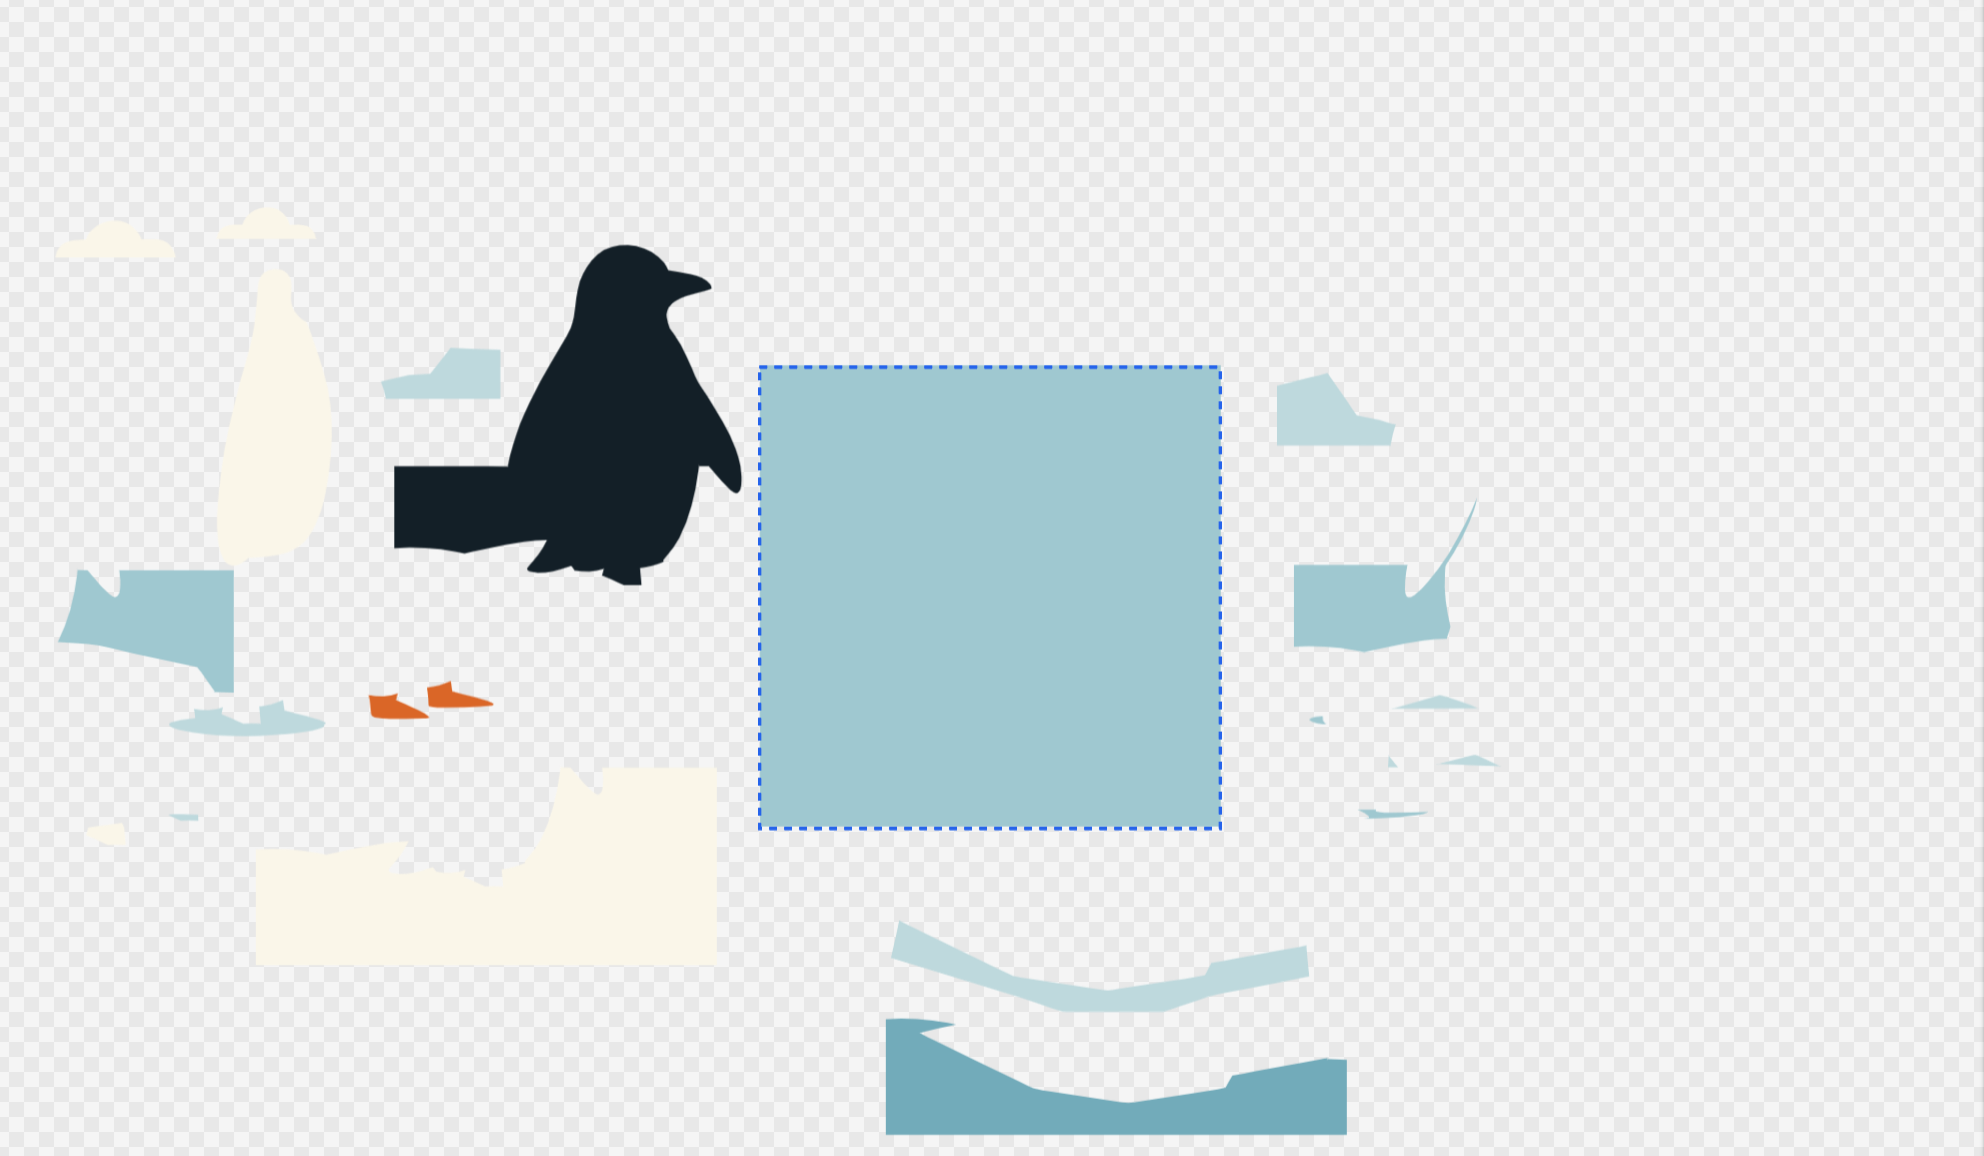
\includegraphics[height=5cm]{svgmaker_sprtd.png} \\
    (a) Rendered output & (b) Elements separated \\
    \end{tabular}
    \caption{SVG generated by SVGMaker.io from the prompt 
    ``a penguin on ice with 16 shapes.'' The rendered output 
    (a) looks visually clean, but separating the elements 
    (b) reveals 24 paths instead of 16, several of which do 
    not correspond to recognizable visual components.}
    \label{fig:svgmaker}
\end{figure}

A systematic comparison of LLM-based SVG generation methods, 
covering both open-source and commercial systems, is a 
natural next step. Malashenko et 
al.~\cite{LeveragingLargeLanguage} provide an initial 
survey of this space.

\chapter{Model Overview Tables}
\label{app:tables}

The tables in this appendix collect the per-model details behind the main 
chapters. They follow the classification in Table~\ref{tab:model_overview} 
and Figure~\ref{fig:taxonomy}.

\begin{landscape}
\section{Task and Inference Overview}
\label{app:task_overview}

\begin{center}
\small
\captionof{table}{Task type, inference mode, input, output, supervision, and core idea of each model.}
\label{tab:app_task_overview}
\begin{tabularx}{\linewidth}{>{\raggedright\arraybackslash}p{2.85cm} >{\raggedright\arraybackslash}p{2.32cm} >{\raggedright\arraybackslash}p{2.10cm} >{\raggedright\arraybackslash}p{1.45cm} >{\raggedright\arraybackslash}p{2.35cm} >{\raggedright\arraybackslash}p{2.35cm} >{\raggedright\arraybackslash}X}
\toprule
\textbf{Model} & \textbf{Task Type} & \textbf{Inference} & \textbf{Input} & \textbf{Output} & \textbf{Supervision} & \textbf{Core Idea} \\
\midrule
VectorFusion & Text-to-SVG & Iterative Opt. & Text & Paths & Semantic & Distills diffusion priors via differentiable rasterization. \\
        SVGFusion & Text-to-SVG & Forward Dec. & Text & Layers/Paths & Supervised & Continuous latent space learning using SVGX dataset. \\
        SVGDreamer & Text-to-SVG & Iterative Opt. & Text & Paths & Semantic & Semantic-driven vectorization (SIVE) and VPSD. \\
        SVGDreamer++ & Text-to-SVG & Iterative Opt. & Text & Paths & Semantic & Hierarchical optimization with adaptive primitive control. \\
        T2V-NPR & Text-to-SVG & Hybrid & Text & Layers/Paths & Sup. + Semantic & Dual-branch VAE learns path latent space constraints. \\
        LayerTracer & Text-to-SVG & Hybrid & Text/Img & Layers/Paths & Supervised & Models designer construction logic via DiT sequences. \\
        Im2Vec & Vectorization & Forward Dec. & Image & Paths & Pixel recon. & Differentiable rasterizer allows learning from appearance. \\
        SAMVG & Vectorization & Iterative Opt. & Image & Paths & Pixel recon. & Uses SAM for semantic initialization in vectorization. \\
        NIVeL & Text-to-SVG & Iterative Opt. & Text & Layers/Paths & Semantic & Implicit neural layers as optimization domain for SDS. \\
        NeuralSVG & Text-to-SVG & Iterative Opt. & Text & Layers/Paths & Semantic & Scene encoded in MLP weights for layered shapes. \\
        LIVE & Vectorization & Iterative Opt. & Image & Paths & Pixel recon. & Layer-wise hierarchical optimization of vector graphics. \\
        DeepSVG & Unconditional & Forward Dec. & None & Paths & Supervised & Hierarchical Transformer for shape/command disentanglement. \\
        DeepIcon & Vectorization & Forward Dec. & Image & Layers/Paths & Supervised & Hierarchical network for direct image-to-SVG translation. \\
\bottomrule
\end{tabularx}
\end{center}
\end{landscape}

\begin{landscape}
\section{Training Architecture: Optimization-Based Methods}
\label{app:arch_opt}

\begin{center}
\small
\captionof{table}{Training architecture of the optimization-based methods.}
\label{tab:app_arch_opt}
\begin{tabularx}{\linewidth}{>{\raggedright\arraybackslash}p{2.85cm} >{\raggedright\arraybackslash}p{2.90cm} >{\raggedright\arraybackslash}p{1.89cm} >{\raggedright\arraybackslash}p{2.32cm} >{\raggedright\arraybackslash}p{3.04cm} >{\raggedright\arraybackslash}p{2.90cm} >{\raggedright\arraybackslash}X}
\toprule
\textbf{Model} & \textbf{Trainables} & \textbf{Training Data} & \textbf{Init.} & \textbf{Supervision} & \textbf{Representation} & \textbf{Priors} \\
\midrule
LIVE & SVG parameters & None & Error-driven & Pixel recon. (UDF + Xing) & Parametric (flat) & None \\
SAMVG & SVG parameters & None & Mask-based & Pixel recon. (MSE + LPIPS) & Parametric (mask-derived) & SAM \\
VectorFusion & SVG parameters & None & Random / Trace & SDS (Stable Diff.) & Parametric (flat) & Stable Diff. \\
SVGDreamer & SVG parameters / LoRA & None & Attention-based (SIVE) & VPSD & Parametric (flat) & Stable Diff. \\
SVGDreamer++ & SVG parameters / LoRA & None & Random + HIVE & VPSD + HIVE loss & Structured parametric & Stable Diff. + SAM \\
NeuralSVG & MLP weights + colors/ LoRA & None & Saliency-based & SDS & Implicit neural fields & Stable Diff. \\
NIVeL & MLP weights + layer colors & None & Random weights & SDS & Implicit neural fields & DeepFloyd \\
Im2Vec\textsuperscript{$\dagger$} & Encoder + RNN + 1D CNN & Raster images & Image encoding & Pixel recon. (raster only) & Parametric paths & None \\
\bottomrule
\end{tabularx}

\vspace{0.5em}
\begin{minipage}{\linewidth}
\footnotesize
\textsuperscript{$\dagger$}Im2Vec is a hybrid (Figure~\ref{fig:taxonomy}). It trains an encoder--decoder using differentiable rendering and reconstruction loss, but at inference there is no iterative refinement. It is placed here because its core contribution is the training objective rather than a learned generative model over SVG structure (see Section~\ref{sec:optimization}).
\end{minipage}
\end{center}
\end{landscape}

\begin{landscape}
\section{Training Architecture: Dataset-Driven Methods}
\label{app:arch_data}

\begin{center}
\small
\captionof{table}{Training architecture of the dataset-driven methods.}
\label{tab:app_arch_data}
\begin{tabularx}{\linewidth}{>{\raggedright\arraybackslash}p{2.85cm} >{\raggedright\arraybackslash}p{3.04cm} >{\raggedright\arraybackslash}p{2.32cm} >{\raggedright\arraybackslash}p{2.32cm} >{\raggedright\arraybackslash}p{2.46cm} >{\raggedright\arraybackslash}p{2.90cm} >{\raggedright\arraybackslash}X}
\toprule
\textbf{Model} & \textbf{Trainables} & \textbf{Training Data} & \textbf{Init.} & \textbf{Supervision} & \textbf{Representation} & \textbf{Priors} \\
\midrule
DeepSVG & VAE (Transformer) weights & SVG-Icons8 & Latent sampling & Recon. + KL & Sequential path tokens & None \\
DeepIcon & Transformer weights & SVG-Icons8 & CLIP embedding & Reconstruction & Sequential path tokens & CLIP encoder \\
SVGFusion & VP-VAE + VS-DiT & SVGX & Random latent & Recon. + Denoising & Continuous latent space & CLIP + DINO-v2 \\
T2V-NPR\textsuperscript{$\dagger$} & NPR-VAE + Latents + LoRA & FIGR-8-SVG & Random path latents & VSD & Neural Path Repr. & Stable Diff. + CLIP \\
LayerTracer & DiT + LoRA & 20k layered SVGs & Diffusion noise & Denoising loss & Layered pixel sequences & Flux DiT + Florence-2 \\
\bottomrule
\end{tabularx}

\vspace{0.5em}
\begin{minipage}{\linewidth}
\footnotesize
\textsuperscript{$\dagger$}T2V-NPR is a hybrid (Figure~\ref{fig:taxonomy}). Its path VAE is trained on FIGR-8-SVG, but at inference the path latents are optimized for each prompt with VSD.
\end{minipage}
\end{center}
\end{landscape}

\begin{landscape}
\section{Reproducibility Overview}
\label{app:reproducibility}

\begin{center}
\small
\captionof{table}{Code availability, pre-trained weights, hardware, time cost, and reproduction feasibility.}
\label{tab:app_reproducibility}
\begin{tabularx}{\linewidth}{>{\raggedright\arraybackslash}p{2.85cm} >{\raggedright\arraybackslash}p{1.52cm} >{\raggedright\arraybackslash}p{3.33cm} >{\raggedright\arraybackslash}p{3.19cm} >{\raggedright\arraybackslash}p{2.75cm} >{\raggedright\arraybackslash}X}
\toprule
\textbf{Model} & \textbf{Code} & \textbf{Pre-trained} & \textbf{Hardware} & \textbf{Cost of time} & \textbf{Reproduction Feasibility} \\
\midrule
LIVE & Yes & No & RTX 3090 & 2,600--10,000 s & Feasible on high-end consumer GPU (slow). \\
SAMVG & No & No & RTX 3090 & 139--2,000 s & Re-implementation possible but requires effort. \\
VectorFusion & No & No & Not specified & 10--20 min & Not reproducible due to lack of public implementation. \\
SVGDreamer & Yes & No & V100 ($\geq$31GB VRAM) & 7--14 min & Requires a high-VRAM GPU; a LoRA is trained during each run. \\
SVGDreamer++ & Yes & No & A800 ($\geq$31GB VRAM) & $\sim$7 min & Requires a high-VRAM GPU; a LoRA is trained during each run. \\
NeuralSVG & Yes & No & Not stated & Unknown & Hardware requirements unclear. \\
NIVeL & Pending & No & A100 & $\sim$5 min & High-end GPU required. \\
T2V-NPR & Yes & VAE (unknown)& RTX 3090 & $\sim$13 min & Feasible on high-end consumer GPU. \\
DeepSVG & Yes & VAE (unknown) & 2×1080Ti (training) & Unknown & Feasible on consumer GPU. \\
DeepIcon & No & Transformer (unknown) & Not specified & -- & Not reproducible (no official code). \\
SVGFusion & No & VP-VAE + VS-DiT (unknown) & Multi-A800 (training) & 24--36 s & No official implementation available. \\
Im2Vec & Yes & VAE (unknown) & Not specified & Unknown & Likely feasible on consumer GPU. \\
LayerTracer & Yes & DiT + LoRA (unknown) & A100 80GB (training) & 27--34 s & Enterprise GPU required. \\
\bottomrule
\end{tabularx}
\end{center}
\end{landscape}

\chapter{Architectural Pipeline Diagrams}
\label{app:pipelines}

The following diagrams visualize the generation pipelines 
of selected models analyzed in this thesis. They are 
grouped by method family to highlight where pipelines 
share components and where they diverge.

\begin{figure}[htbp]
    \centering
    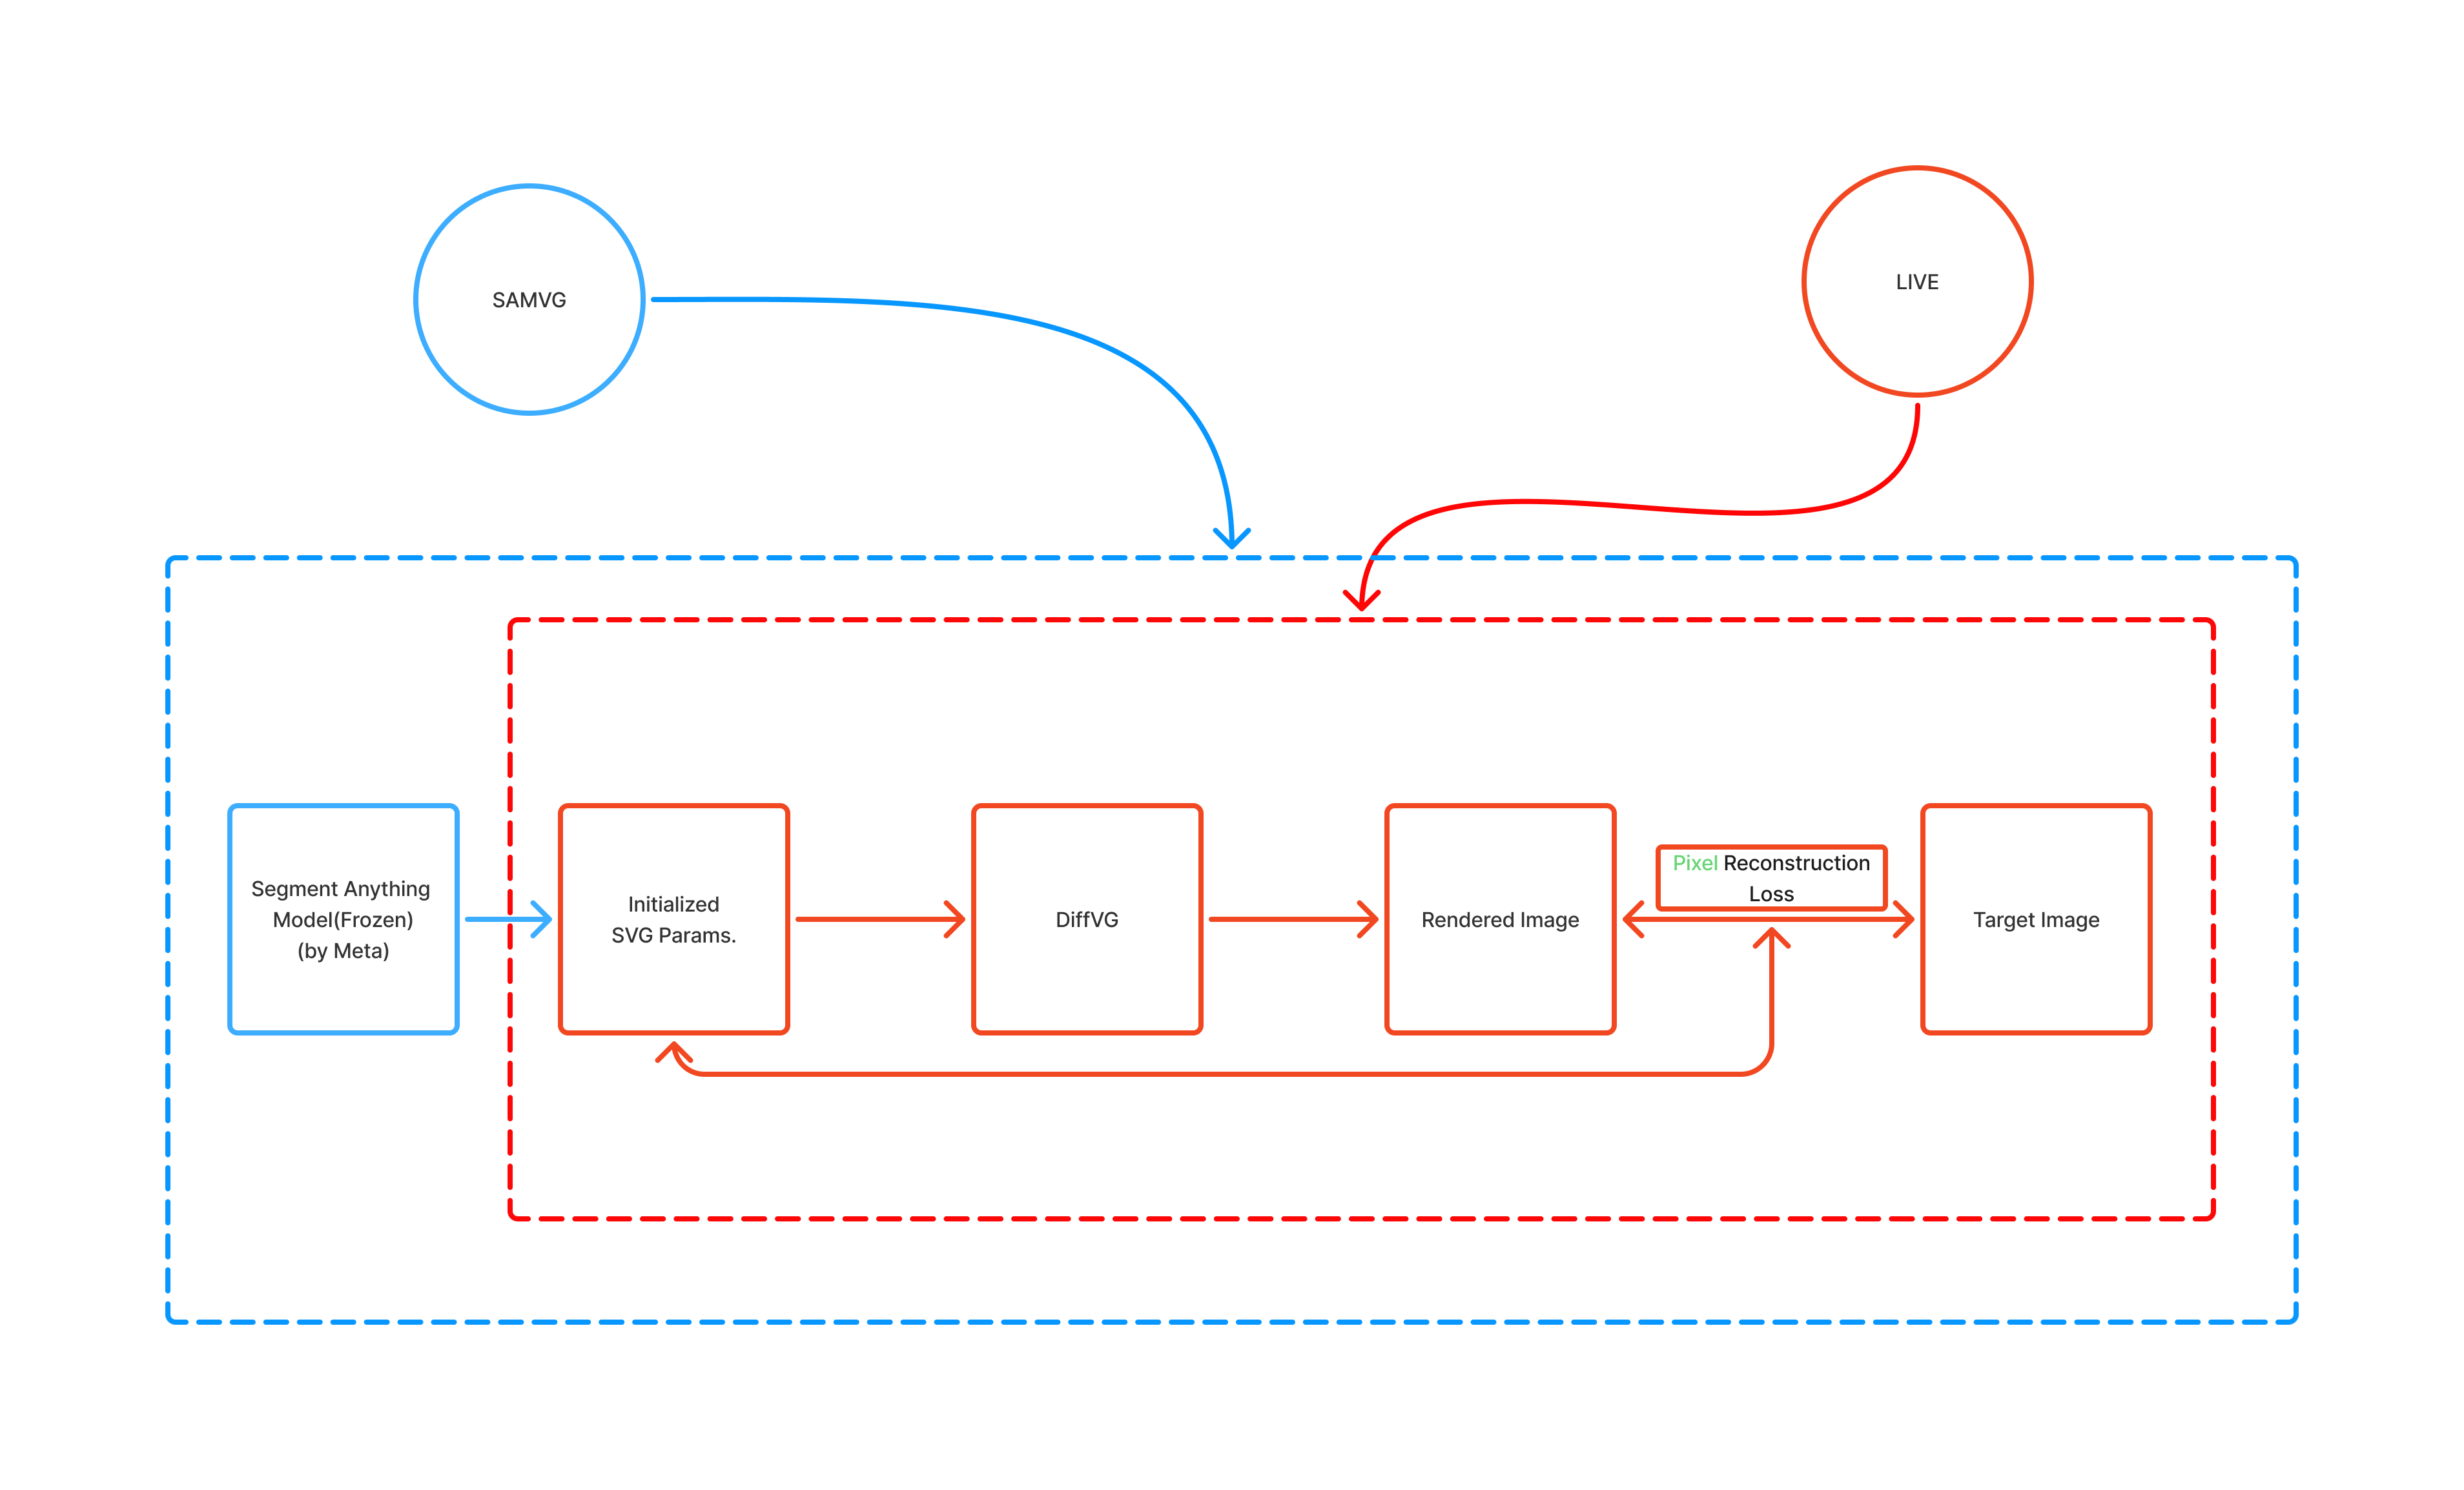
\includegraphics[width=\textwidth]{LIVEnSAM.png}
    \caption{Reconstruction-supervised optimization pipelines. 
    LIVE (red) and SAMVG (blue) share the same core loop: 
    Initialized SVG Params $\rightarrow$ DiffVG $\rightarrow$ 
    Rendered Image $\rightarrow$ Pixel Reconstruction Loss 
    $\rightarrow$ Target Image, with gradients flowing back 
    to update the SVG parameters. The main difference is 
    where optimization starts. LIVE initializes directly 
    from the target image through residual analysis. SAMVG 
    adds the Segment Anything Model as a preprocessing step, 
    producing semantically meaningful initialization regions 
    before the same optimization loop begins. Same kind of loss, 
    different starting point, different structural outcome.}
    \label{fig:opt_recon_pipelines}
\end{figure}

\begin{figure}[htbp]
    \centering
    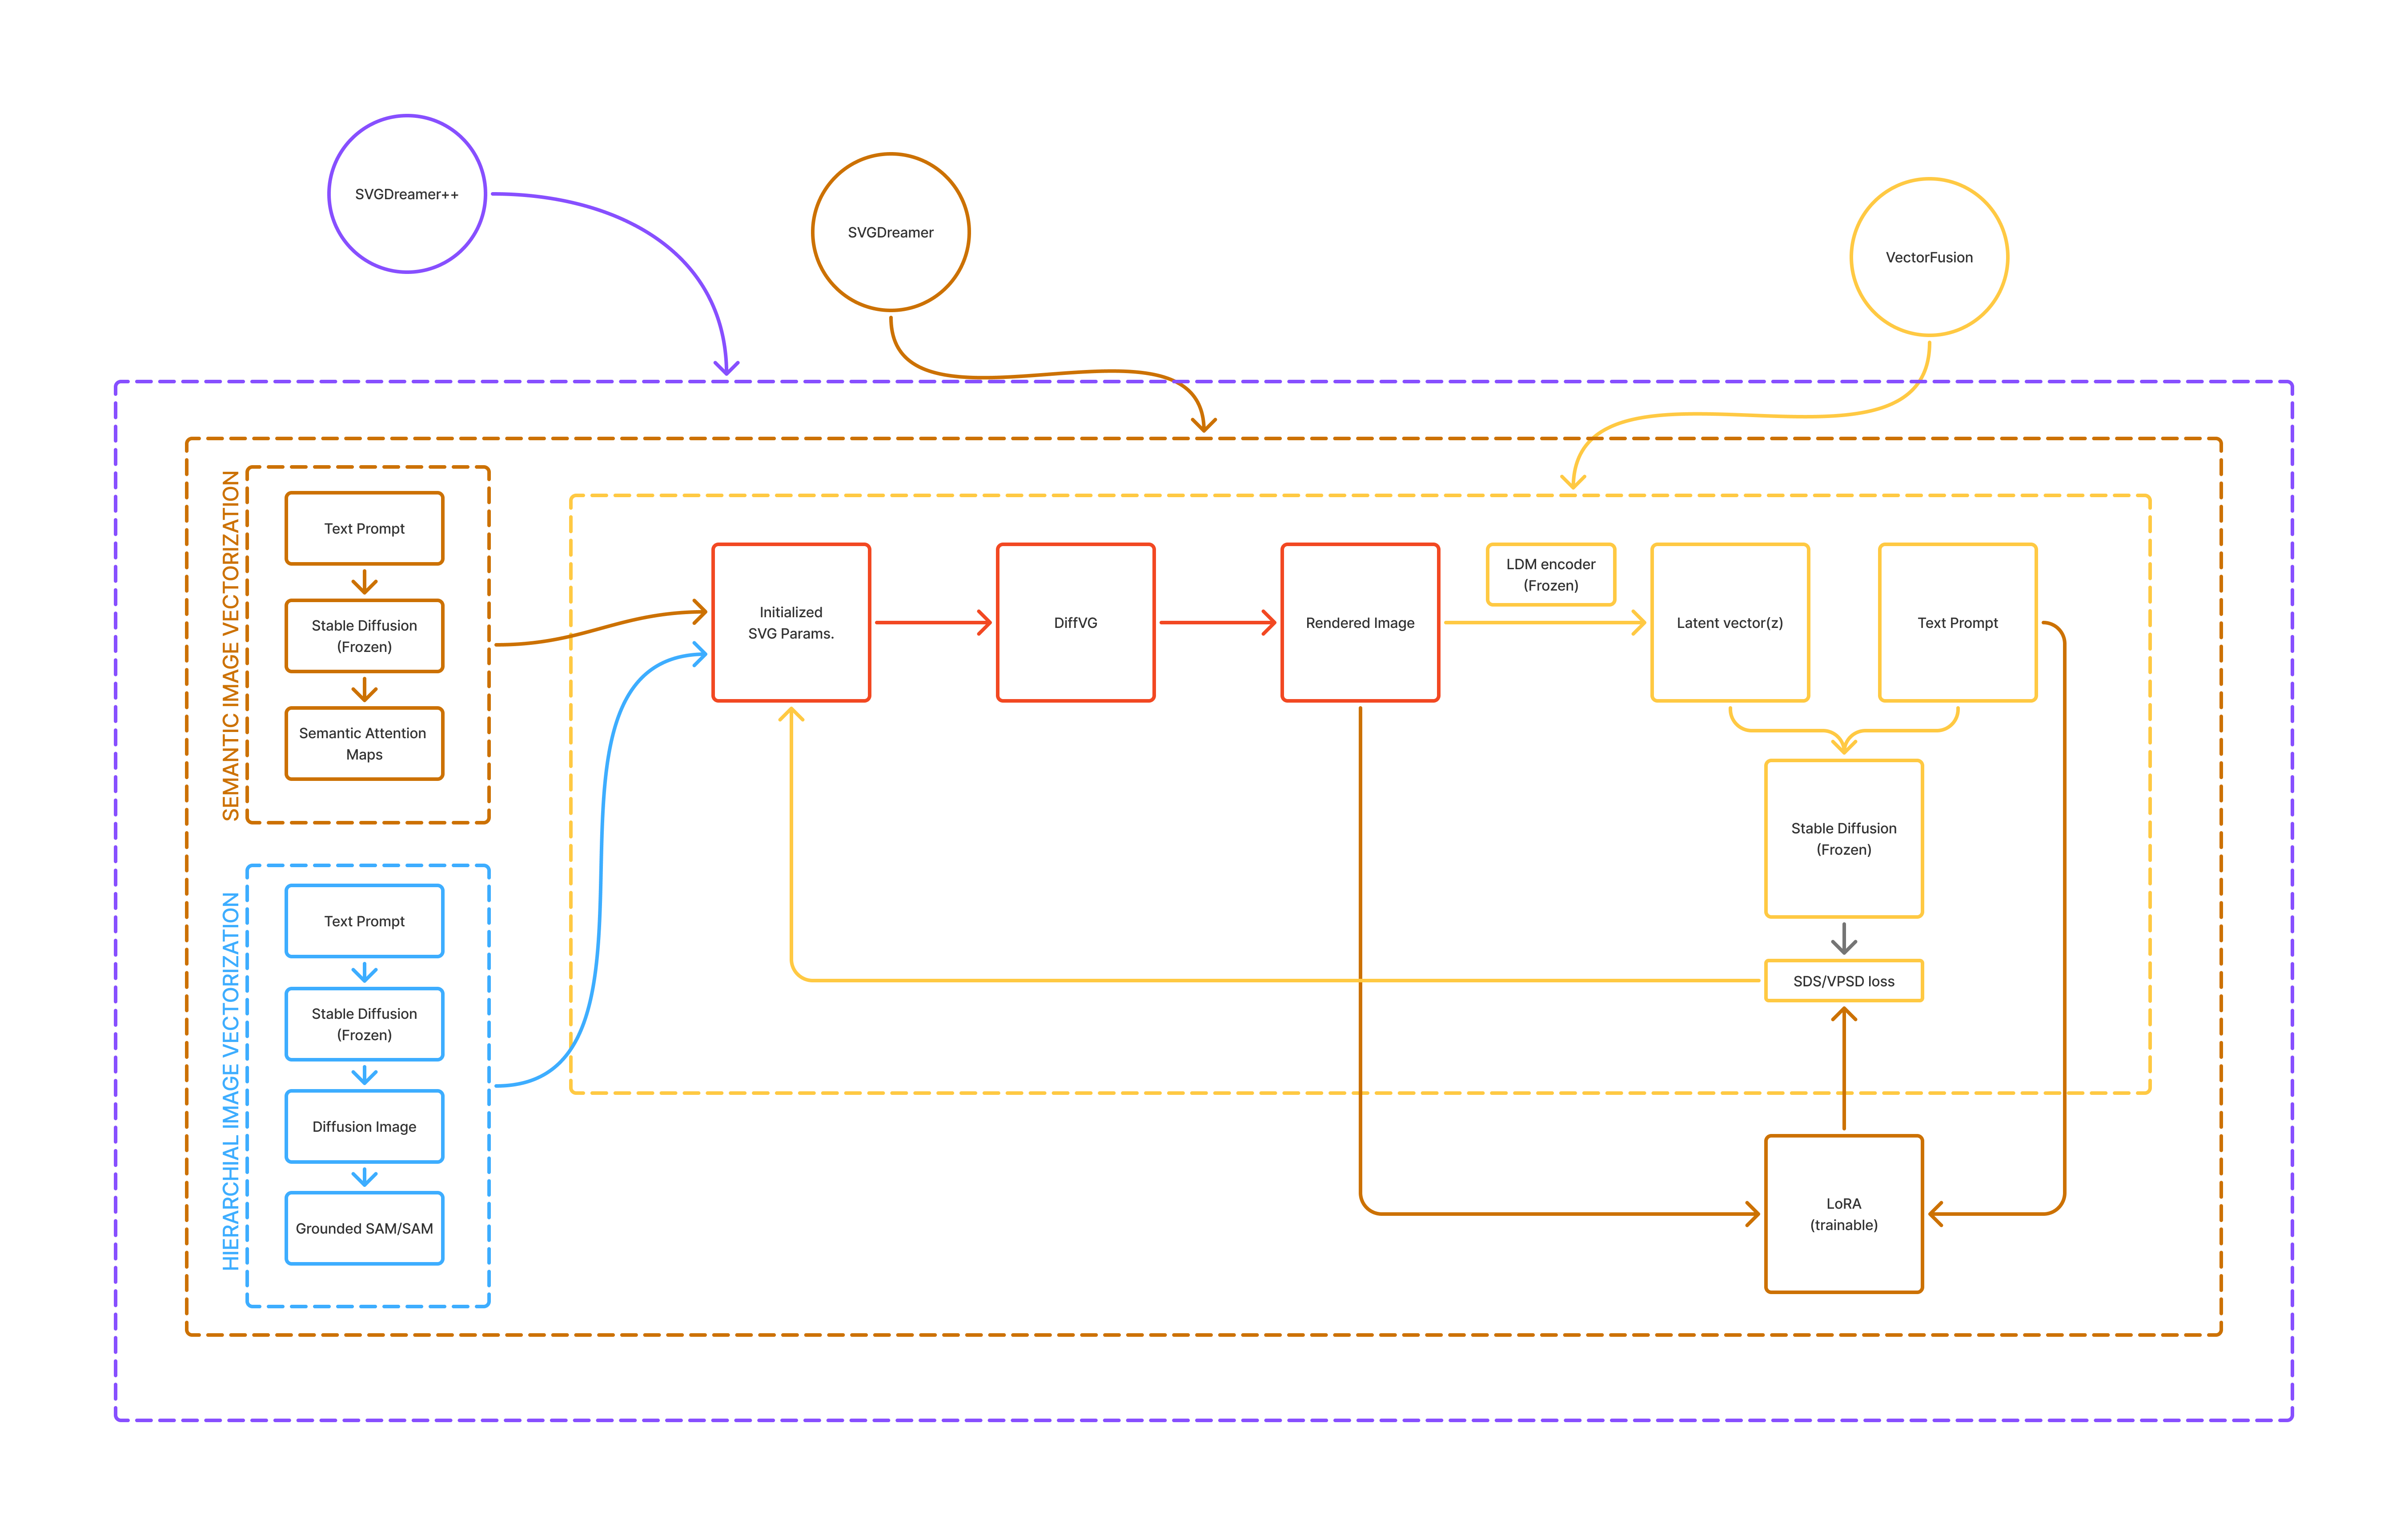
\includegraphics[width=\textwidth]{OPT..png}
    \caption{Semantic-supervised optimization pipelines. 
    VectorFusion (orange), SVGDreamer (orange with blue 
    SIVE initialization), and SVGDreamer++ (purple, adding 
    hierarchical image vectorization via Grounded SAM). All 
    three share the same core optimization loop (Initialized 
    SVG Params $\rightarrow$ DiffVG $\rightarrow$ Rendered 
    Image $\rightarrow$ SDS/VPSD loss) but differ in how 
    primitives are initialized and what additional supervision 
    signals are applied. SVGDreamer adds semantic attention 
    maps for initialization. SVGDreamer++ replaces those 
    with Grounded SAM for finer part-level decomposition.}
    \label{fig:opt_semantic_pipelines}
\end{figure}

\begin{figure}[htbp]
    \centering
    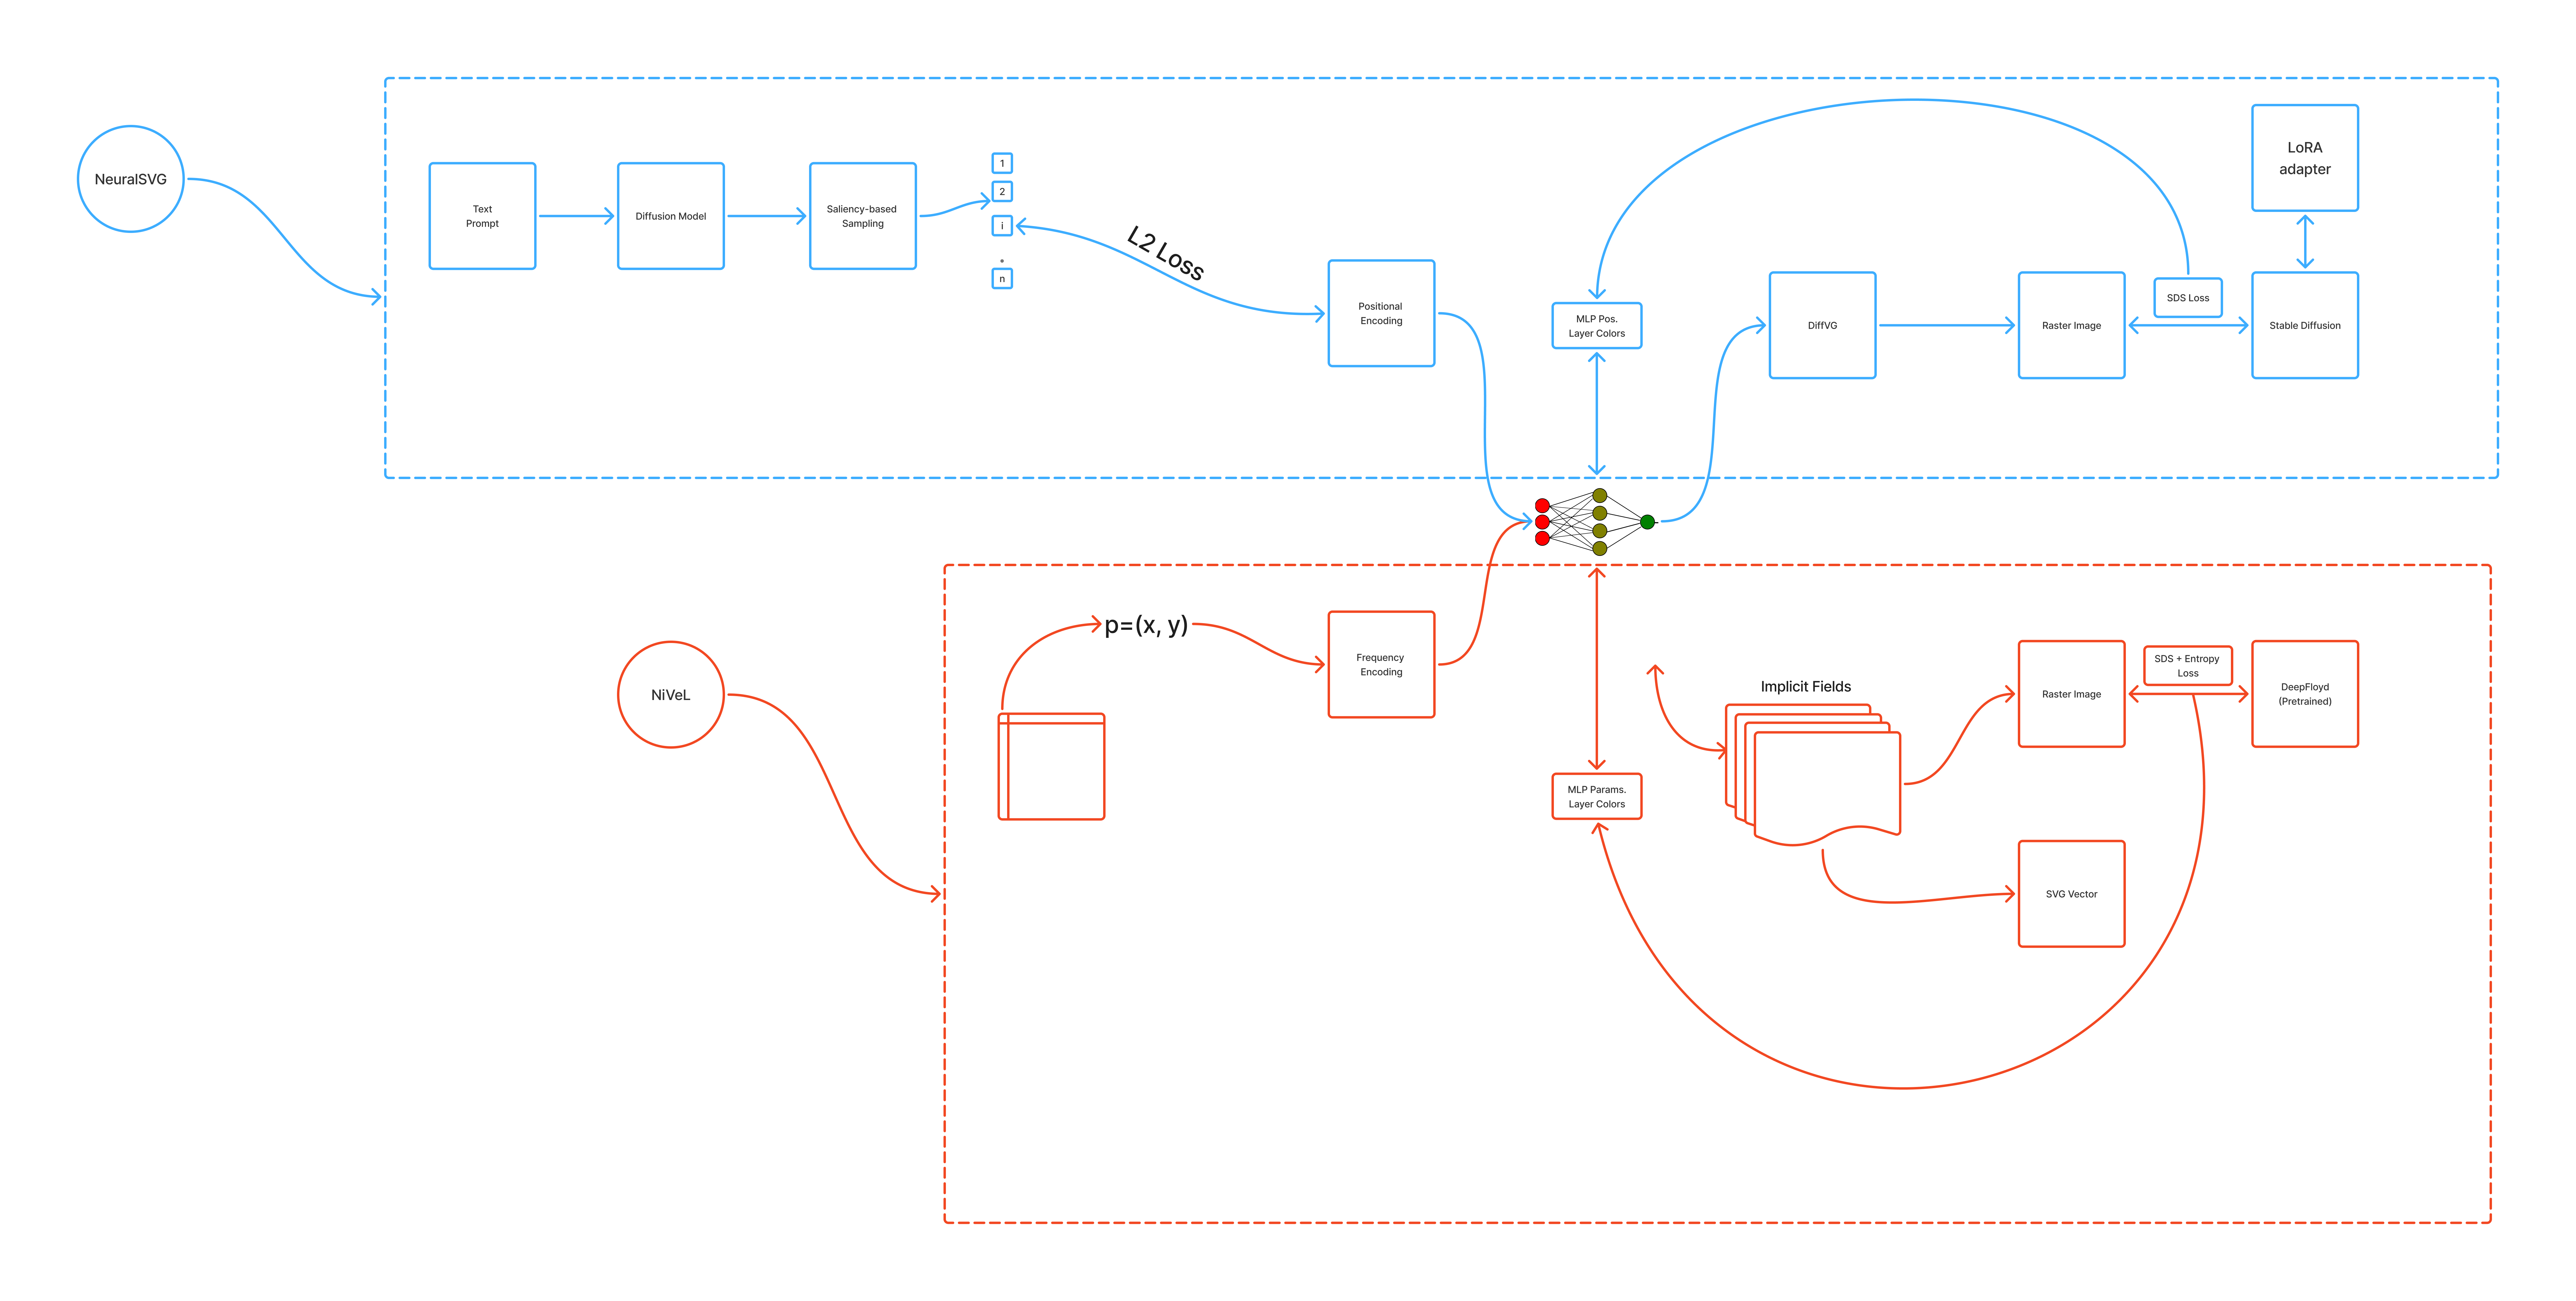
\includegraphics[width=\textwidth]{OPT.+NN.png}
    \caption{Neural implicit optimization pipelines. 
    NeuralSVG (blue) and NIVeL (red) both store geometry 
    in MLP weights rather than explicit B\'{e}zier 
    coordinates, but their pipelines differ. NeuralSVG 
    generates an initial layout through saliency-based 
    sampling from a diffusion model, encodes shape indices 
    via positional encoding, and optimizes MLP weights 
    using SDS loss with a LoRA adapter on Stable Diffusion. 
    NIVeL takes spatial coordinates as input, applies 
    frequency encoding, and optimizes layered implicit 
    fields using SDS with entropy loss through DeepFloyd. 
    Both produce SVG output by converting the learned 
    implicit representation into discrete vector primitives.}
    \label{fig:opt_neural_pipelines}
\end{figure}




    \backmatter


    % this you need to sign and include the signed pdf
    % Magda Gregorova, 2025-01-10

\addchap{Declaration on oath}

I hereby certify that I have written my master thesis independently and have not yet submitted it for examination purposes elsewhere.
All sources and aids used are listed, literal and meaningful quotations have been marked as such.

\vspace{40pt}
\begin{flushright}
  \rule{5cm}{0.4pt}\\
  April 14, 2026, \ShowThesisAuthor    
\end{flushright}

\addchap{Consent to plagiarism check}

I hereby agree that my submitted work may be sent to PlagAware (https://my.plagaware.com/) in digital form for the purpose of checking for plagiarism and that it may be temporarily (max. 5~years) stored in the database maintained by PlagScan as well as personal data which are part of this work may be stored there.

\begin{small}
Consent is voluntary.
Without this consent, the plagiarism check cannot be prevented by removing all personal data and protecting the copyright requirements.
Consent to the storage and use of personal data may be revoked at any time by notifying the faculty.
\end{small}

\begin{flushright}
  \rule{5cm}{0.4pt}\\
  April 14, 2026, \ShowThesisAuthor    
\end{flushright}
    \end{document}
